\appendix
\section{Domain Details}
\label{appendix:domain}
See an overview of the six domains we use in our experiments in \cref{fig:env_renders}.
We also include the dataset size, episode length and the action dimension in Table \ref{tab:metadata}. In the following sections, we describe each domain in details.



\subsection{OGBench environments.} We consider five manipulation domains from OGBench~\citep{ogbench_park2024} and take the publicly available single-task versions of it in our experiments. For \texttt{scene-sparse} and \texttt{puzzle-3x3-sparse}, we sparsify the reward function such that the reward values are $-1$ when the task is incomplete and $0$ when the task is completed. For \texttt{cube-double/triple/quadruple}, the RL agent needs to command an UR-5 arm to pick and place two/three/four cubes to target locations. In particular, \texttt{cube-triple} and \texttt{cube-quadruple} are extremely difficult to solve from offline data only, and often achieve zero success rate. The RL agent must explore efficiently online in these domains to solve the tasks. The \texttt{cube-*} domains provide a great test ground for sample-efficiency of offline-to-online RL algorithms which we primarily focus on. For \texttt{cube-quadruple}, we use the 100M-size dataset. The dataset is too big to fit our CPU memory, so we periodically (after every 1000 gradient steps) load in a $1$M-size chunk of the dataset for offline training. For online training of \hourblue{RLPD}, \hourpurple{QC-RLPD}, we use the same strategy where we load in a $1$M-size chunk of the dataset as the offline data and perform 50/50 sampling (e.g., 50\% of the data comes from the $1$M-chunk of the offline data, 50\% of the data comes from the online replay buffer). For online fine-tuning of \hourpurple{QC-*}, \hourblue{FQL}, \hourblue{FQL-n}, \hourblue{BFN}, and \hourblue{BFN-n}, we keep a fixed $1$M-size chunk of the offline dataset as the initialization of $\mathcal{D}$ and adds new data to $\mathcal{D}$ directly. The remaining $99$M transitions in the offline data are not being used online. We now describe each of the five domains in details:

\texttt{scene-sparse}: This domain involves a drawer, a window, a cube and two button locks that control whether the drawer and the window can be opened. These tasks typically involve a sequence of actions. For example, \texttt{scene-task2} requires the robotic arm to unlock both locks, move the drawer and the window to the desired position, and then lock both locks. \texttt{scene-task4} requires the robotic arm to unlock the drawer, open the drawer, put the cube into the drawer, close the drawer. The reward is binary: $-1$ if the desired configuration is not yet reached and $0$ if the desired configuration is reached (and the episode terminates).

\texttt{puzzle-3x3-sparse}: This domain contains a $3\times3$ grid of buttons. Each button has two states represented by its color (blue or red). Pressing any button causes its color and the color of all its adjacent buttons to flip (red $\rightarrow$ blue and blue $\rightarrow$ red). The goal is to achieve a pre-specified configuration of colors. \texttt{puzzle-3x3-task2} starts with all buttons to be blue, and the goal is to flip exactly one button (the top-left one) to be red. \texttt{puzzle-3x3-task4} starts with four buttons (top-center, bottom-center, left-center, right-center) to be blue, and the goal is to turn all the buttons to be blue. The reward is binary: $-1$ if the desired configuration is not yet reached and $0$ if the desired configuration is reached (and the episode terminates).


\texttt{cube-double/triple/quadruple}: These three domains contain 2/3/4 cubes respectively. The tasks in the three domains all involve moving the cubes to their desired locations.
The reward is $-n_{\mathrm{wrong}}$ where $n_{\mathrm{wrong}}$ is the number of the cubes that are at the wrong position. The episode terminates when all cubes are at the correct position (reward is 0).

\subsection{Robomimic environments.} We use three challenging tasks from the robomimic domain~\citep{robomimic2021}.
We use the multi-human datasets that were collected by six human operators. Each dataset contains 300 successful trajectories. The three tasks are as described as follows.
\begin{itemize}
    \item \texttt{lift}: This task requires the robot arm to pick a small cube. This is the simplest task of the benchmark.
    \item \texttt{can}: This task requires the robot arm to pick up a coke can and place in a smaller container bin.
    \item \texttt{square}: This task requires the robot arm to pick a square nut and place it on a rod. The nut is slightly bigger than the rod and requires the arm to move precisely to complete the task successfully.
\end{itemize}

All of the three robomimic tasks use binary task completion rewards where the agent receives $-1$ reward when the task is not completed and $0$ reward when the task is completed.

\begin{table}[ht]
    \centering
    \begin{tabular}{@{}cccc@{}}
        \toprule
        \textbf{Tasks} & \textbf{Dataset Size}  & \textbf{Episode Length} & \textbf{Action Dimension ($A$)} \\
        \midrule
        \texttt{scene-sparse-*}       &  $1$M & $750$ & $5$\\
        \texttt{puzzle-3x3-sparse-*}  &  $1$M & $500$ & $5$\\
        \texttt{cube-double-*} &  $1$M & $500$ & $5$\\
        \texttt{cube-triple-*} &  $3$M & $1000$ & $5$\\
        \texttt{cube-quadruple-100M-*} &  $100$M & $1000$ & $5$\\
        \texttt{lift}        &  $31\,127$& $500$ & $7$\\
        \texttt{can}        &  $62\,756$ & $500$ & $7$\\
        \texttt{square}        &  $80\,731$ & $500$ & $7$\\
    \bottomrule
    \end{tabular}
    \vspace{2mm}
    \caption{\footnotesize \textbf{Domain metadata.} Dataset size (number of transitions), episode length, and the action dimension. For OGBench tasks, the action dimension is 5 ($x$ position, $y$ position, $z$ position, gripper yaw and gripper opening). For robomimic tasks, the action dimension is 7 for square to control one arm (3 degree of freedoms (DoF) for translation, 3 DoF for rotation, and one final DoF for the gripper opening).}

    \label{tab:metadata}
\end{table}



\begin{figure*}[t]
    \centering
    \begin{minipage}{0.24\textwidth}
        \begin{subfigure}{\textwidth}
            \centering
            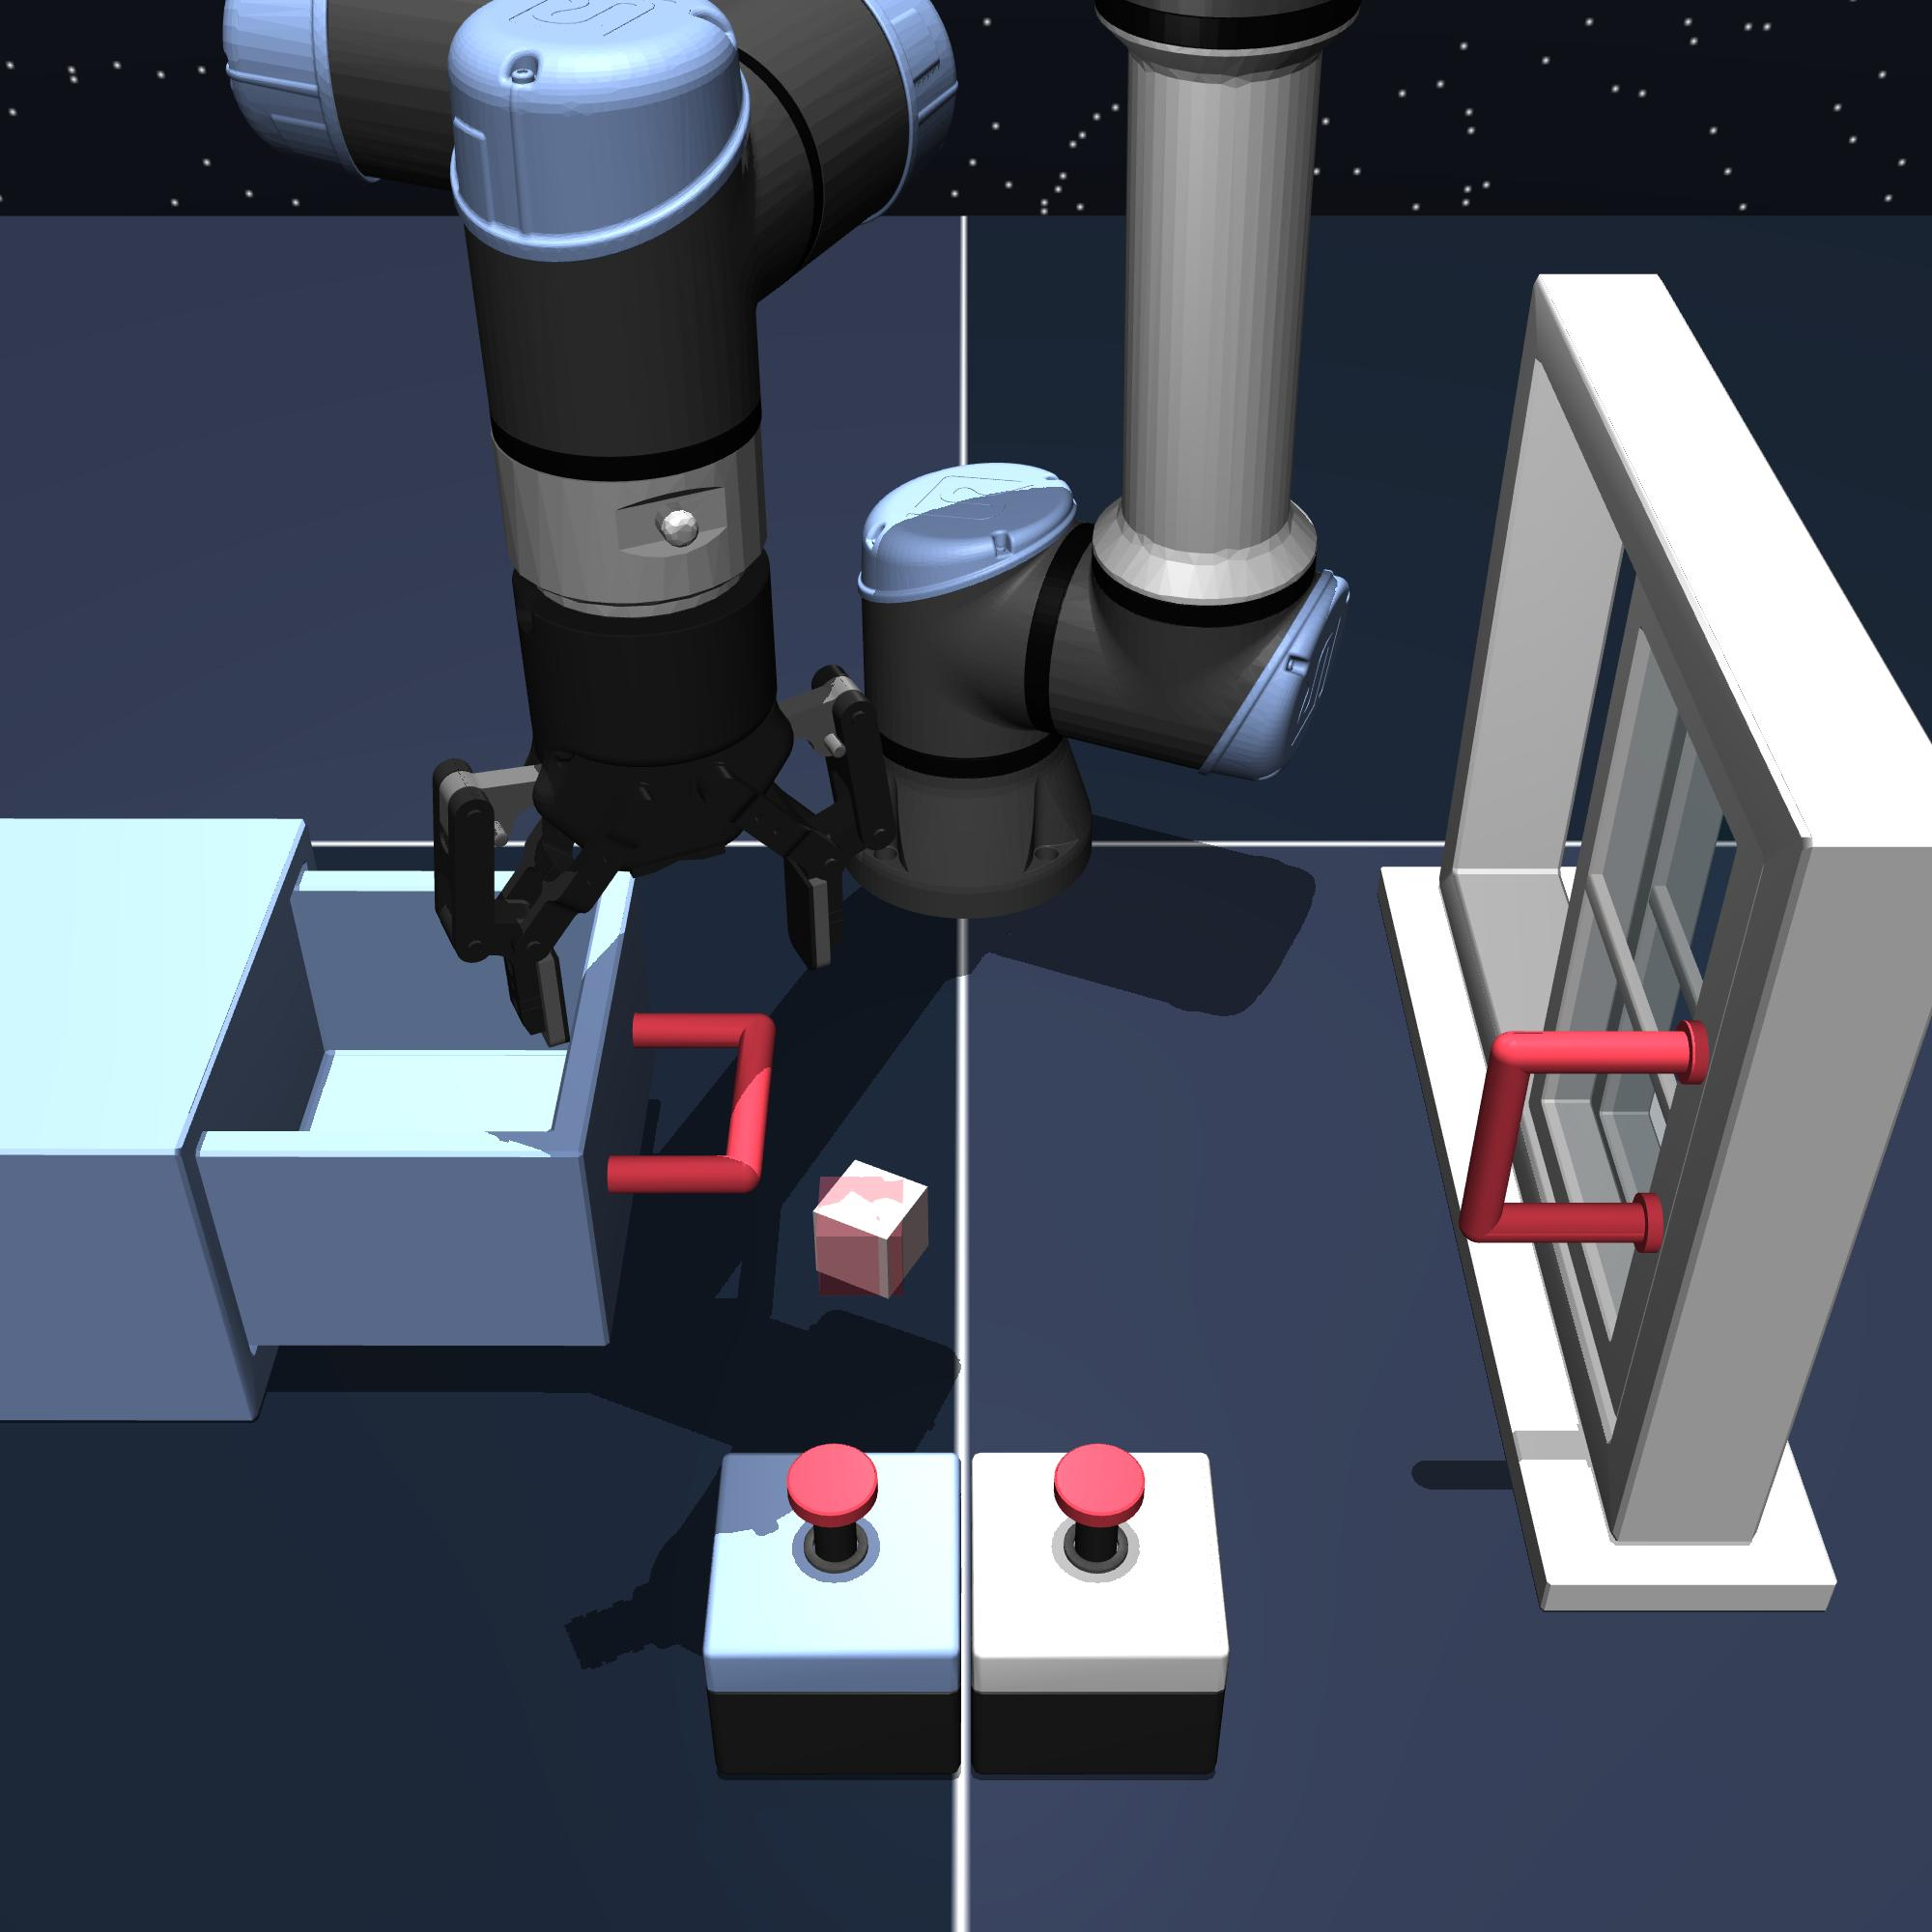
\includegraphics[width=0.98\textwidth]{figures/renders/scene-play-singletask-task2-v0.jpeg}
            \caption{\footnotesize a) \texttt{scene}}
            \label{fig:scene-viz}
        \end{subfigure}
    \end{minipage}\hfill
    \begin{minipage}{0.24\textwidth}
        \begin{subfigure}{\textwidth}
            \centering
            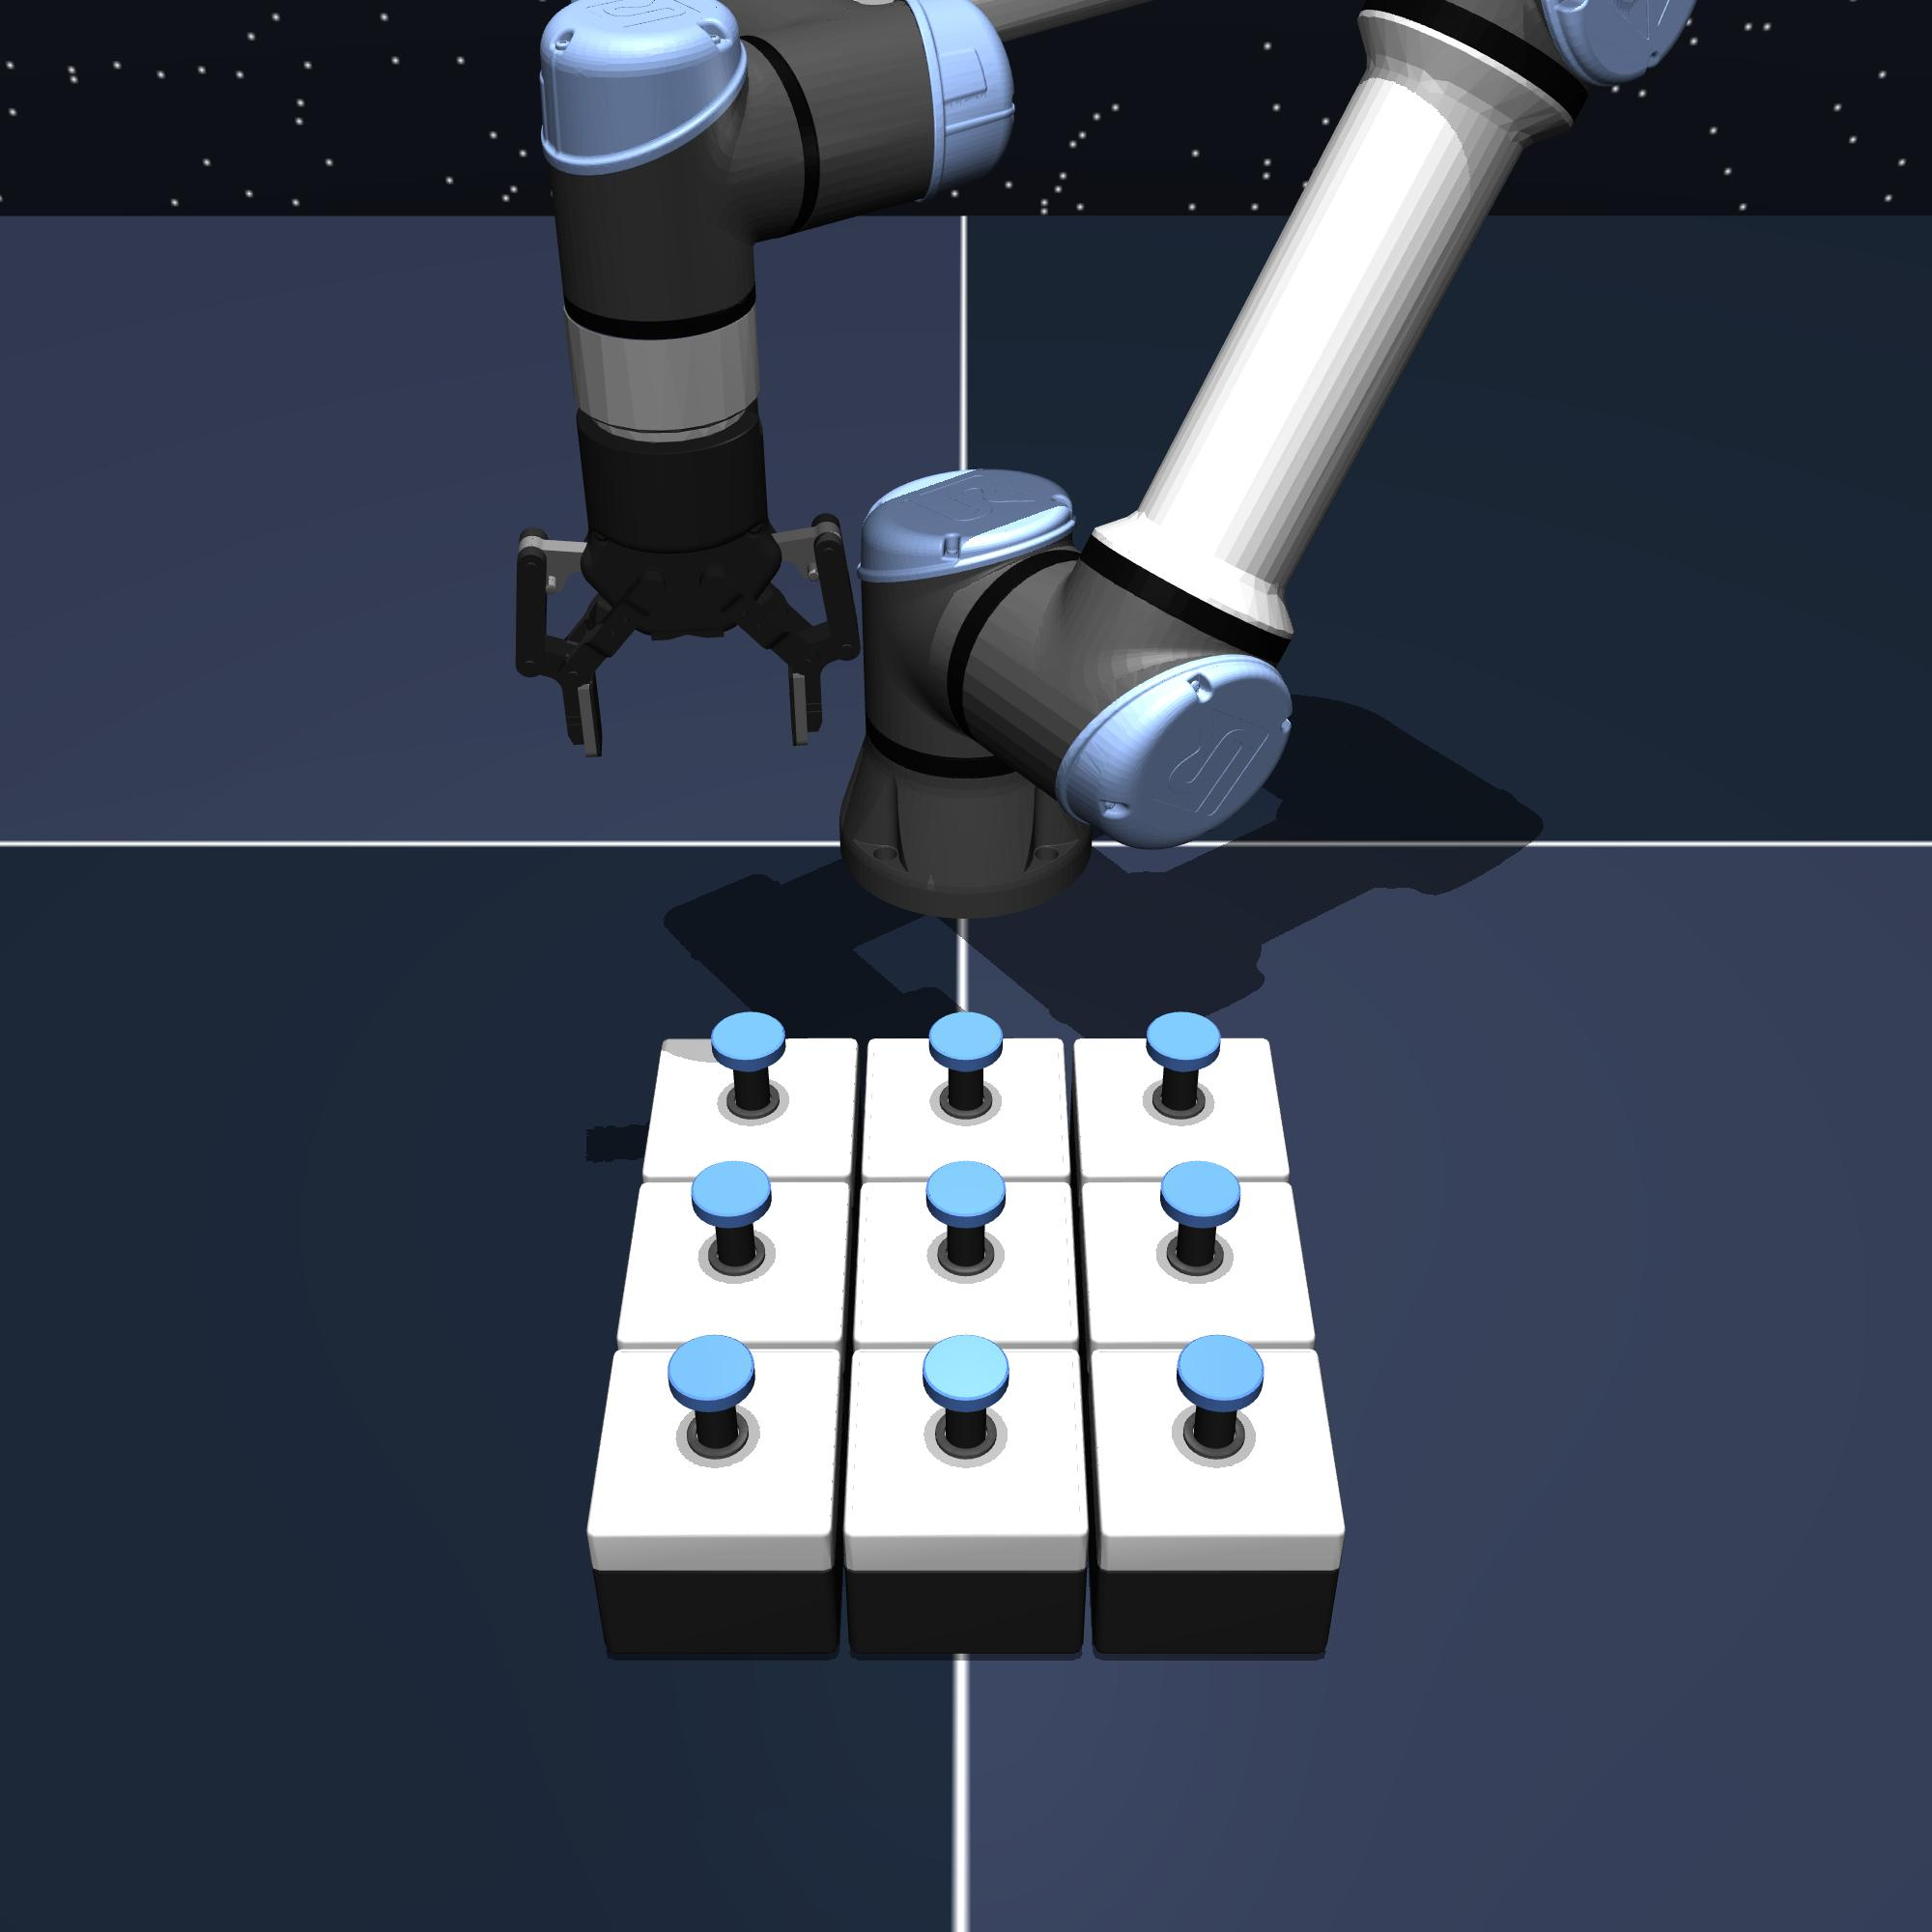
\includegraphics[width=0.98\linewidth]{figures/renders/puzzle-3x3-play-singletask-task2-v0.jpeg}
            \caption{\footnotesize b) \texttt{puzzle-3x3}}
            \label{fig:puzzle-viz}
        \end{subfigure}
    \end{minipage}\hfill
    \begin{minipage}{0.24\textwidth}
        \begin{subfigure}{\textwidth}
            \centering
            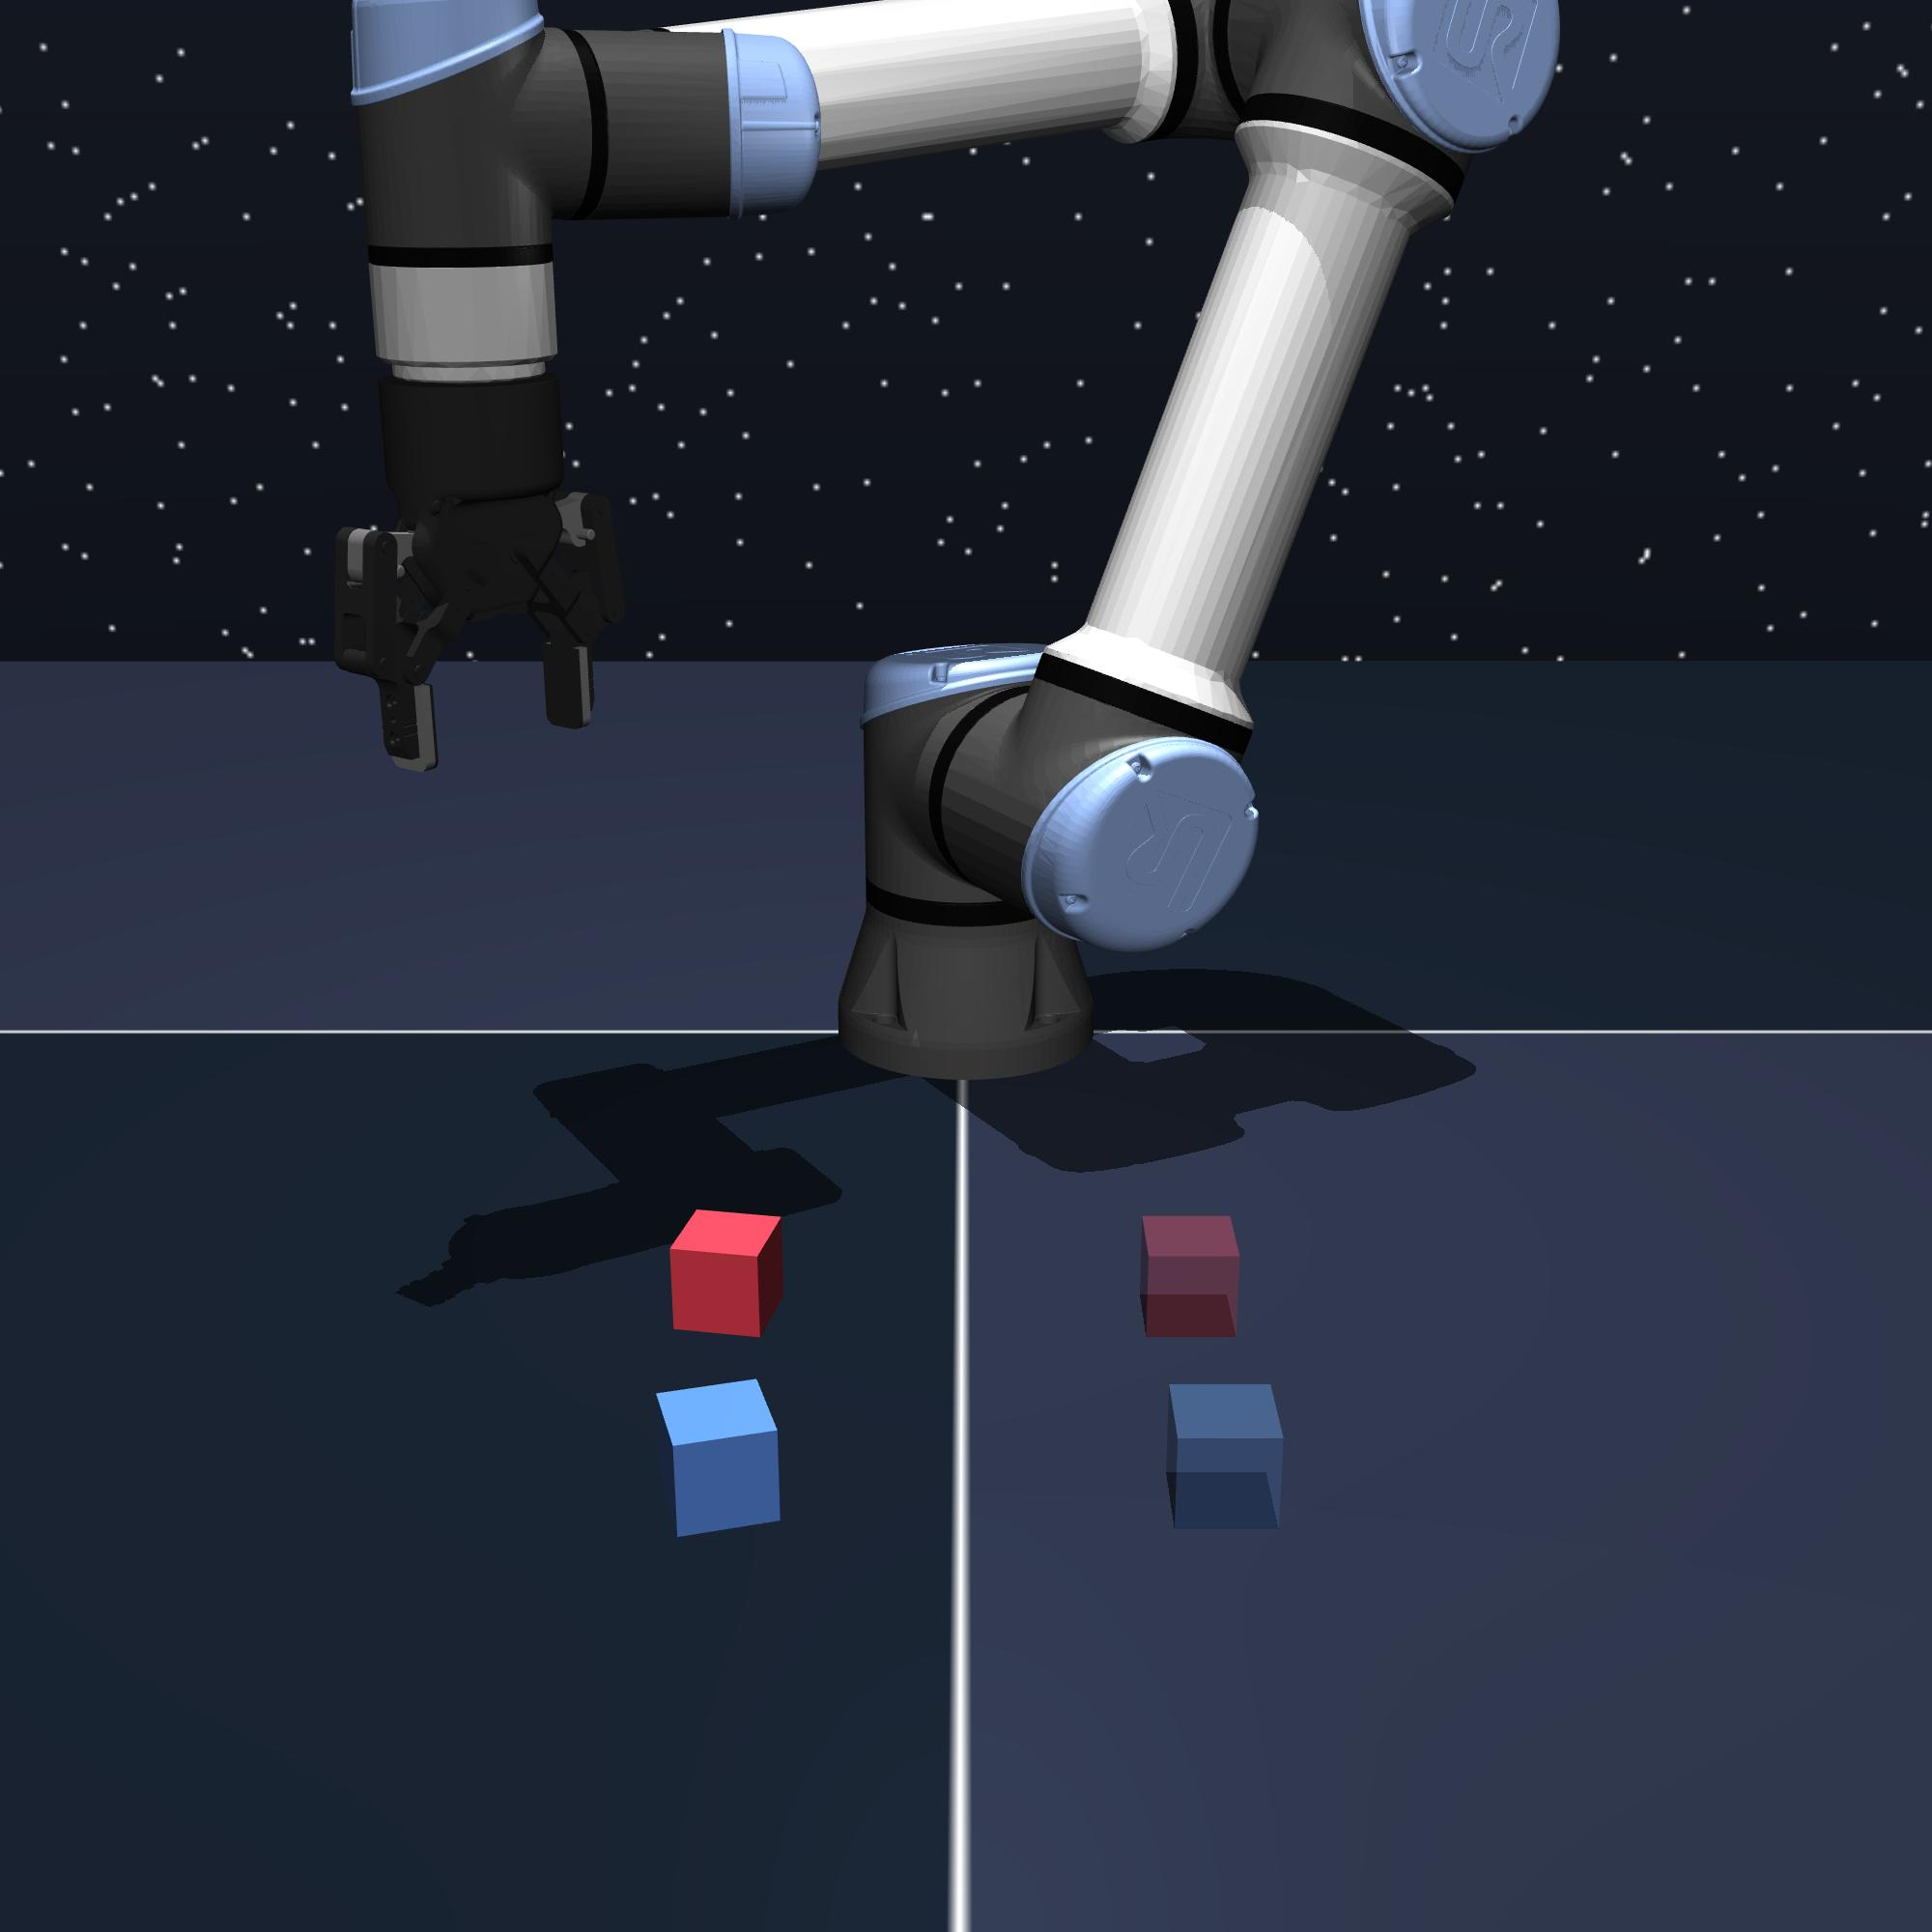
\includegraphics[width=0.98\textwidth]{figures/renders/cube-double-play-singletask-task2-v0.jpeg}
            \caption{\footnotesize c) \texttt{cube-double}}
            \label{fig:cube-double-viz}
        \end{subfigure}
    \end{minipage}\hfill
    \begin{minipage}{0.24\textwidth}
        \begin{subfigure}{\textwidth}
            \centering
            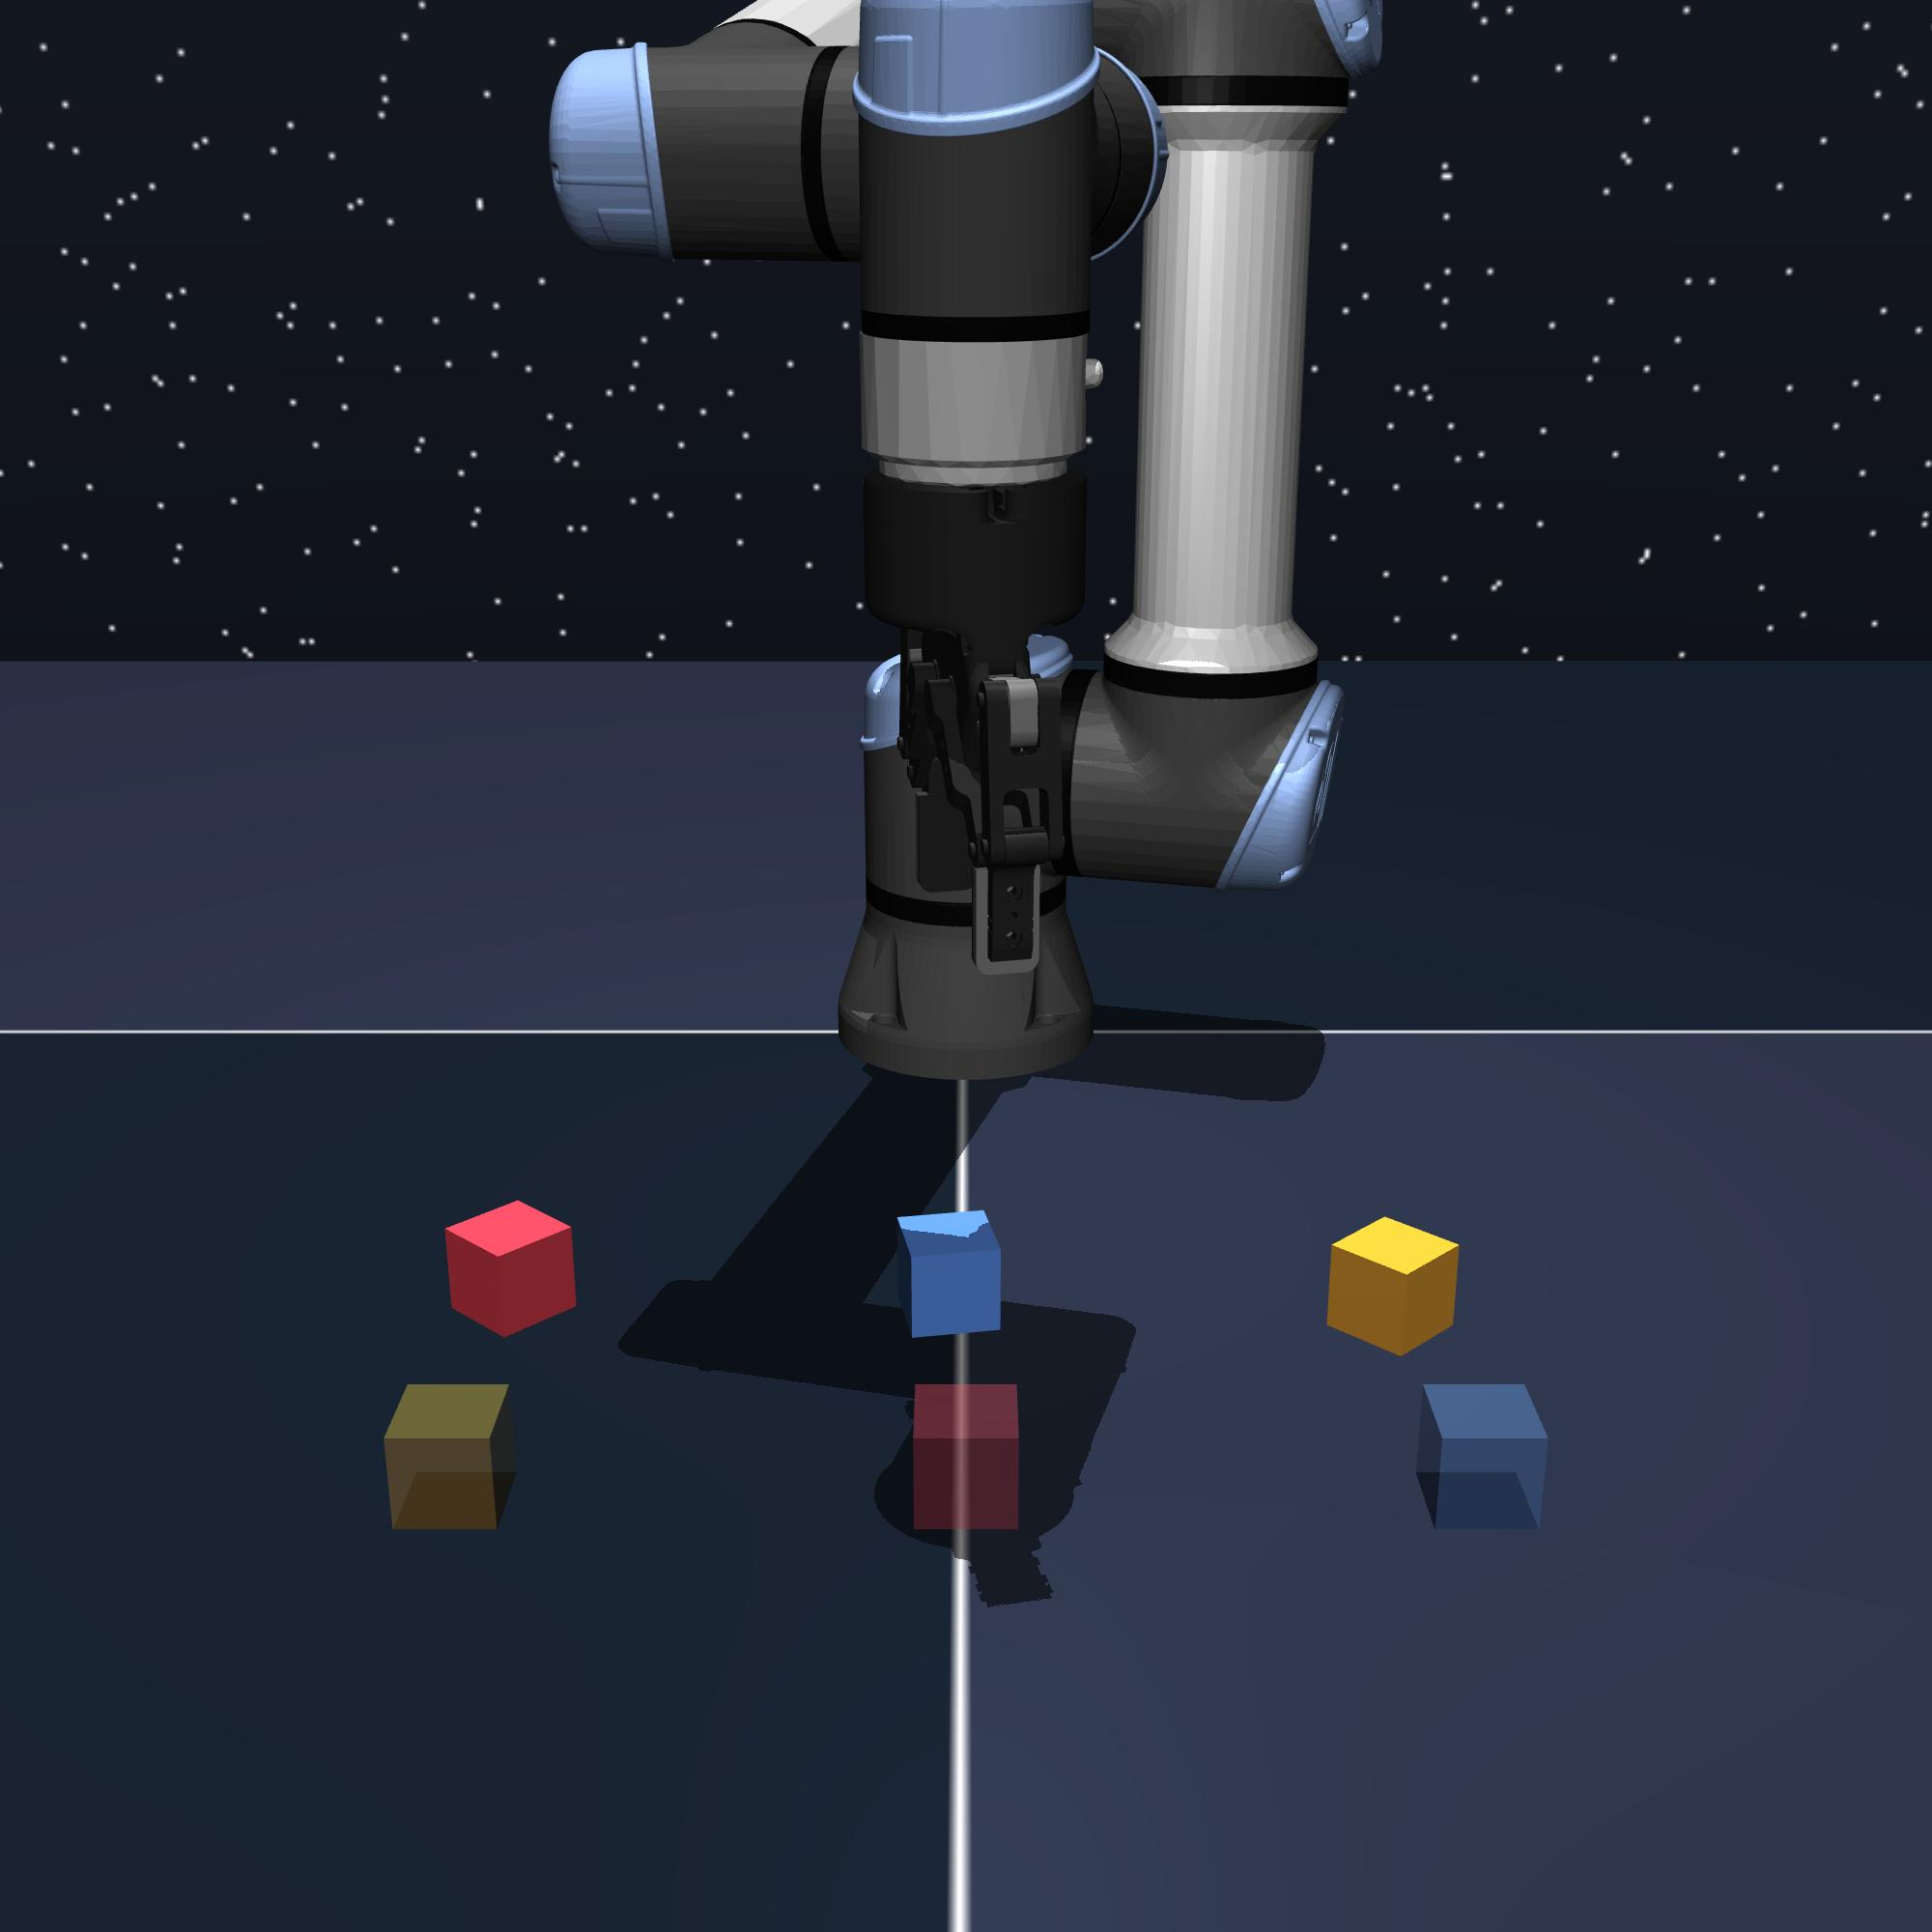
\includegraphics[width=0.98\linewidth]{figures/renders/cube-triple-play-singletask-task2-v0.jpeg}
            \caption{\footnotesize d) \texttt{cube-triple}}
            \label{fig:cube-triple-viz}
        \end{subfigure}
    \end{minipage}

    \begin{minipage}{0.24\textwidth}
        \begin{subfigure}{\textwidth}
            \centering
            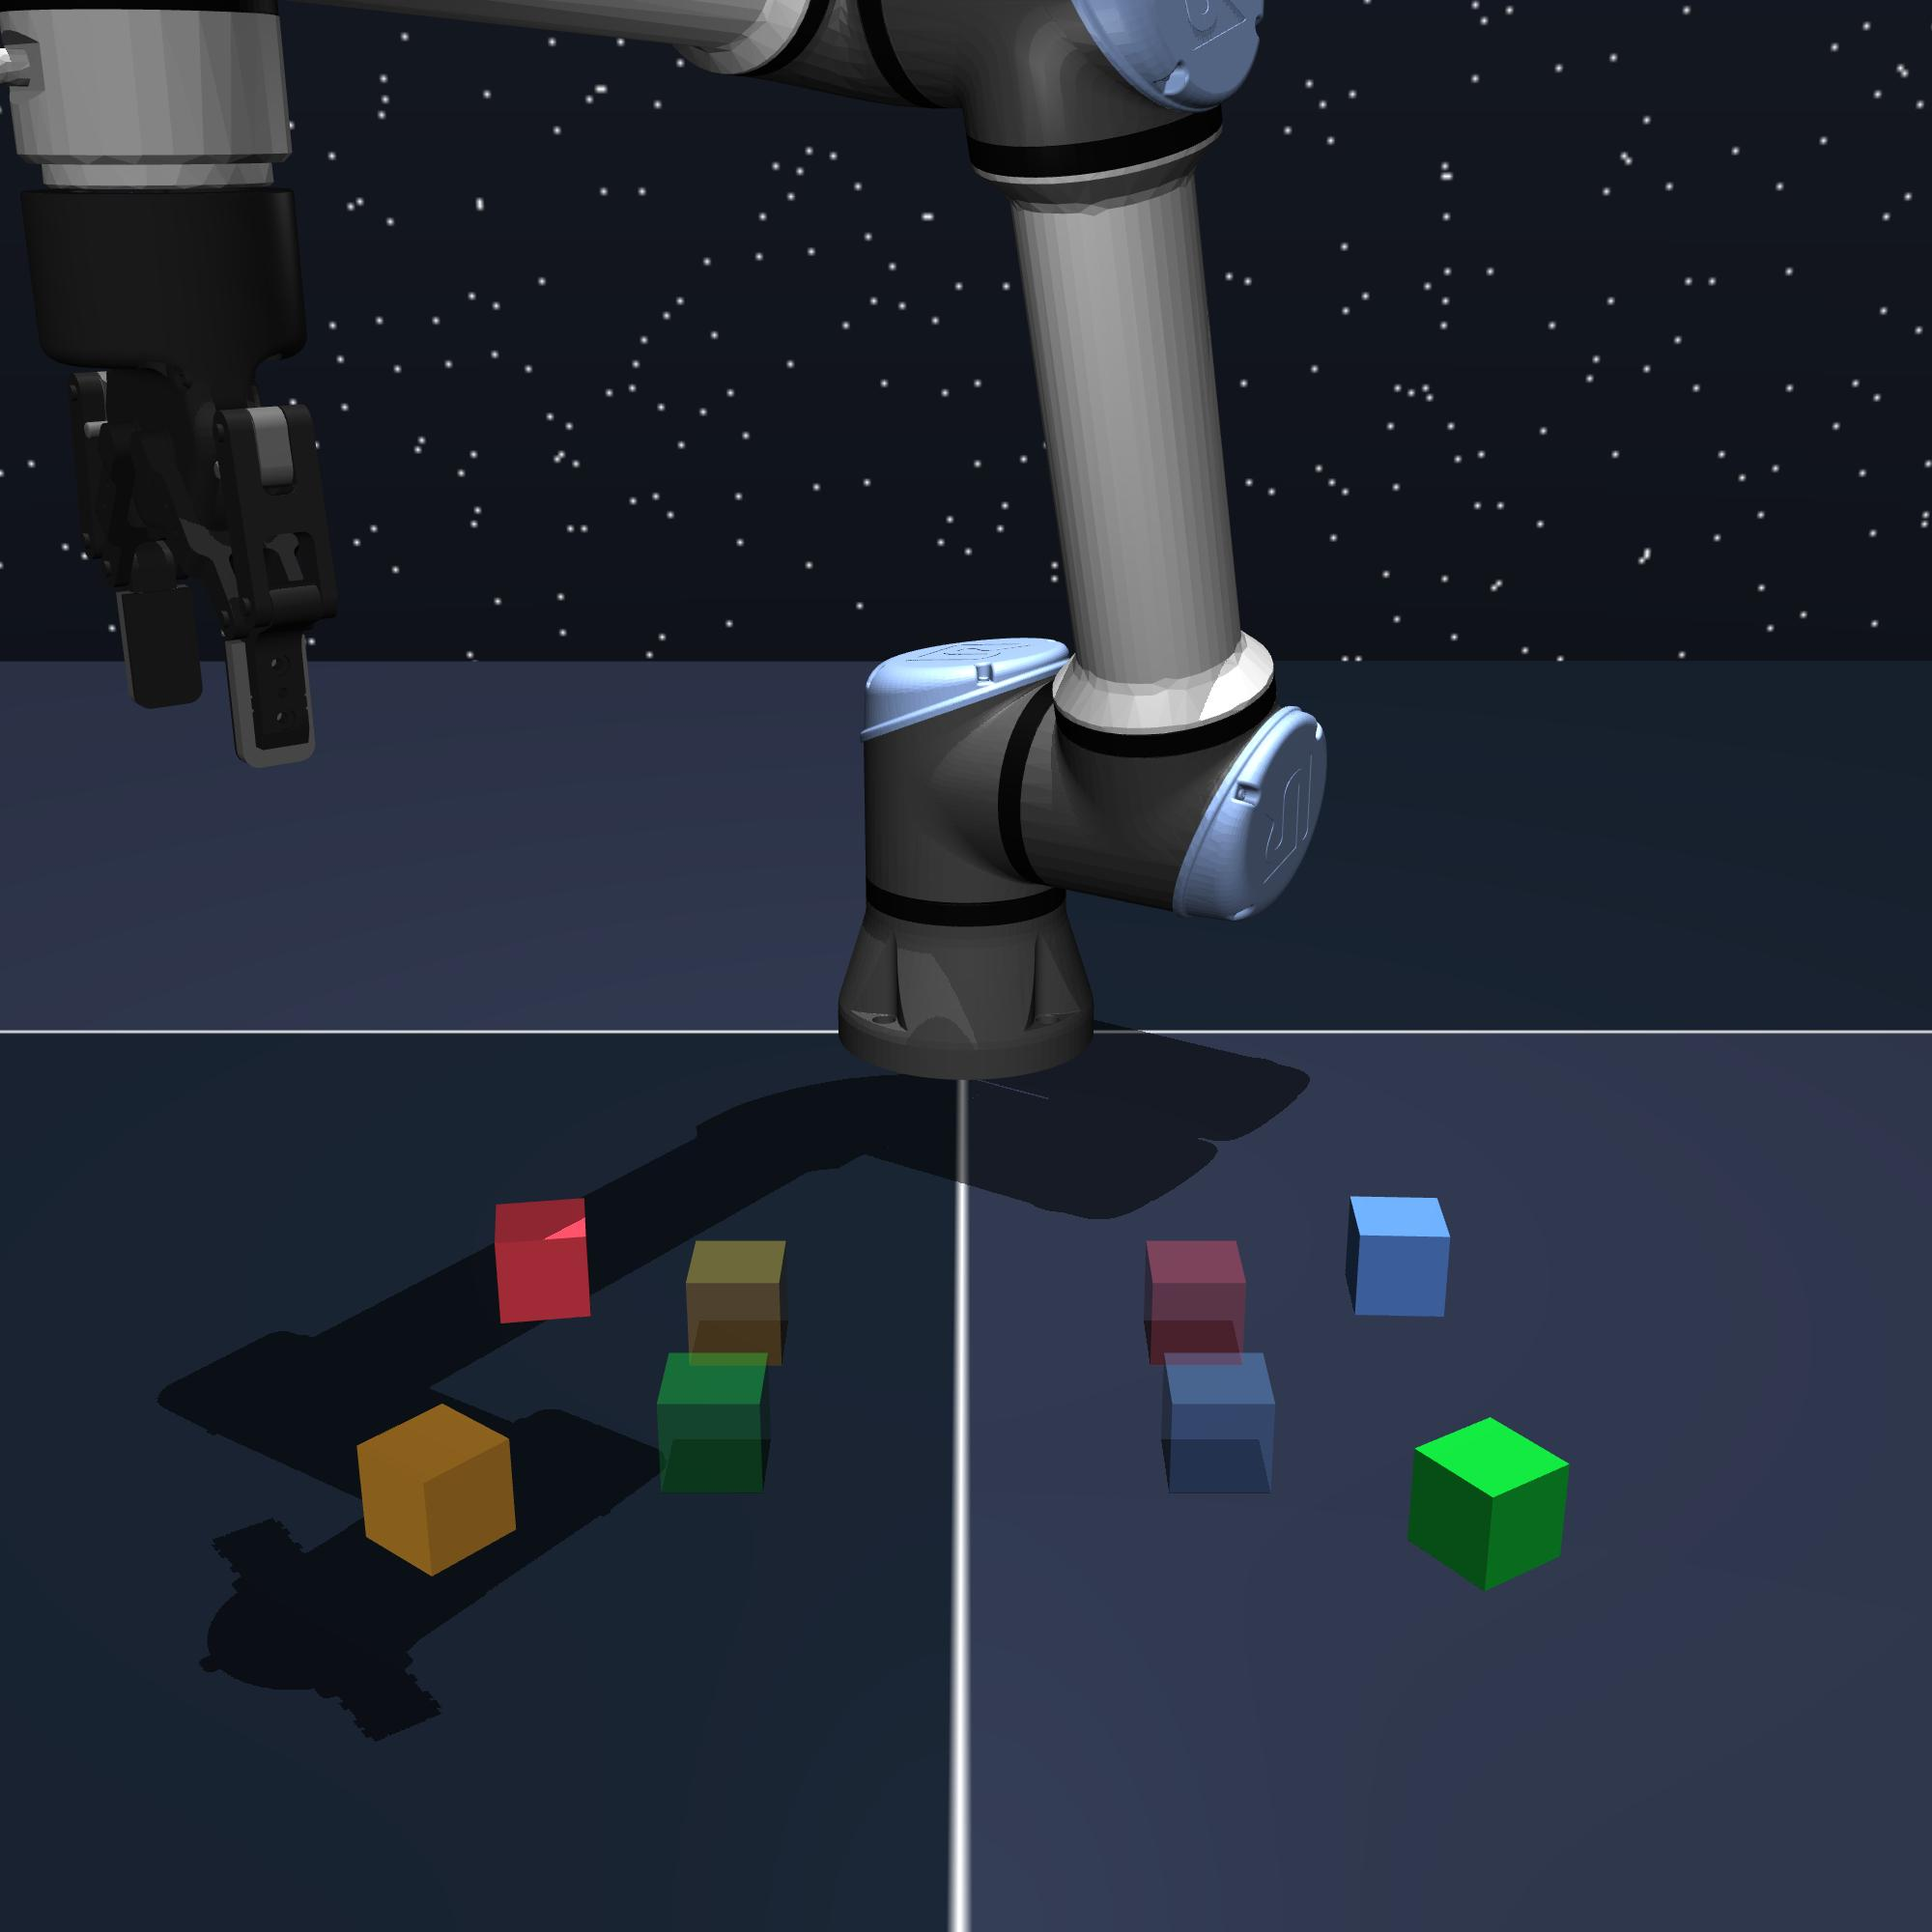
\includegraphics[width=0.98\linewidth]{figures/renders/cube-quadruple-play-singletask-task2-v0.jpeg}
            \caption{\footnotesize e) \texttt{cube-quadruple}}
            \label{fig:cube-quadruple-viz}
        \end{subfigure}
    \end{minipage}\hfill
    \begin{minipage}{0.24\textwidth}
        \begin{subfigure}{\textwidth}
            \centering
            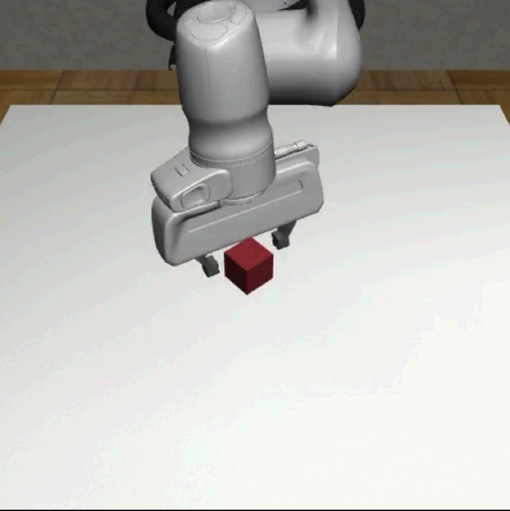
\includegraphics[width=\linewidth]{figures/renders/lift.jpeg}
            \caption{\footnotesize f) \texttt{lift}}
        \end{subfigure}
    \end{minipage}\hfill
    \begin{minipage}{0.24\textwidth}
        \begin{subfigure}{\textwidth}
            \centering
            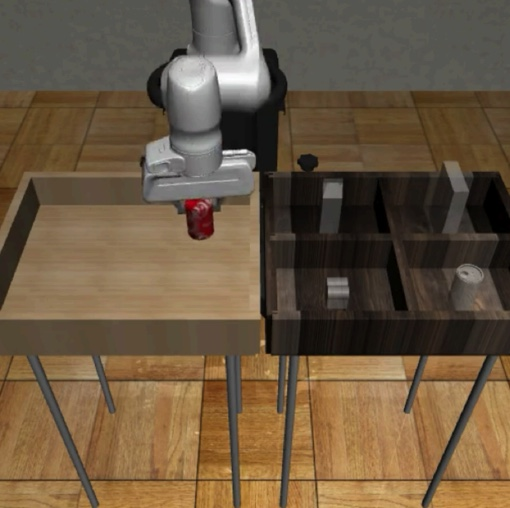
\includegraphics[width=\linewidth]{figures/renders/can.jpeg}
            \caption{\footnotesize g) \texttt{can}}
        \end{subfigure}
    \end{minipage}\hfill
    \begin{minipage}{0.24\textwidth}
        \begin{subfigure}{\textwidth}
            \centering
            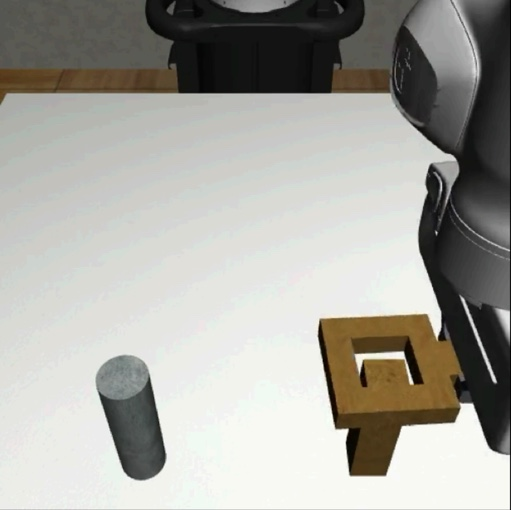
\includegraphics[width=\linewidth]{figures/renders/square.jpeg}
            \caption{\footnotesize h) \texttt{square}}
        \end{subfigure}
    \end{minipage}\hfill
    \caption{\footnotesize \textbf{We experiment on several challenging long-horizon, sparse-reward domains.} See detailed task description for each domain in Appendix \ref{appendix:domain}. The rendered images of the robomimic tasks above are taken from \citet{robomimic2021}.}
    \label{fig:env_renders}
\end{figure*}




\section{Implementation Details}
\label{appendix:impl-details}
In this section, we provide more implementation details on both of our Q-chunking methods and all our baselines used in our experiments.





\subsection{\hourpurple{QC-FQL}}
We build the implementation of our method on top of \hourblue{FQL}~\citep{park2025flow}, a recently proposed offline RL/offline-to-online RL method that uses TD3+BC-style objective. It is implemented with a one-step noise-conditioned policy (instead of a Gaussian policy that is commonly used in RL) and it uses a distillation loss from a behavior flow-matching policy as the BC loss. To adapt this method to use action chunking, we simply apply \hourblue{FQL} on the temporally extended action space -- the behavior flow-matching policy generates a sequence of actions, the one-step noise-conditioned policy predicts a sequence of actions, and the $Q$-network also takes in a state and a sequence of actions. More concretely, we train three networks:
\begin{enumerate}
    \item $Q_\theta(s, a_1, \cdots a_h): \mathcal{S}\times \mathcal{A}^h \mapsto \mathbb{R}$ --- the value function that takes in a state and a sequence of actions (action chunk). In practice, we train an ensemble of $Q$ networks. We denote the weight of the ensemble element as $\theta = (\theta_1, \cdots, \theta_K)$.
    \item $\mu_\psi(s, z): \mathcal{S}\times \mathbb{R}^{Ah} \mapsto \mathbb{R}^{Ah}$ --- the one-step noise-conditioned policy that takes in a state and a noise, and outputs a sequence of actions conditioned on them.
    \item $f_\xi(s, m, u): \mathcal{S} \times \mathbb{R}^{Ah} \times [0, 1] \mapsto \mathbb{R}^{Ah}$ --- the flow-matching behavior policy parameterized by a velocity prediction network. The network predicts takes in a state, an intermediate state of the flow and a time, and outputs the velocity direction that the intermediate action sequence should move in at the specified time. See \cref{algo:flow-step} for more details on how this velocity prediction network is used to generate an action from a noise vector.
\end{enumerate}
We denote our policy as $\pi_\psi(\cdot|s)$. It is implemented by first sampling a Gaussian noise $z \sim \mathcal{N}(0, I_{Ah})$ and run it through the one-step noise-conditioned policy $\begin{bmatrix} a_1 & \cdots & a_h \end{bmatrix} \leftarrow \mu_\psi(s, z)$. To train these three networks, we sample a high-level transition, $w = (s_t, a_t, a_{t+1}, \cdots, a_{t+h-1}, s_{t+h}, r^h_t) \sim \mathcal{D}$ where $r^h_t = \sum_{t'=0}^{h-1}\gamma^{t'}r_{t+t'}$, to construct the following losses:



\textbf{(1) Critic loss:}
\begin{align}
    L(\theta_k, w) = \left(Q_{\theta_k}(s_t, a_t, \cdots, a_{t+h-1}) - r^h_t - \frac{1}{K}\sum_{k'=1}^{K} Q_{\bar \theta_{k'}}(s_{t+h}, a_{t+h}, \cdots, a_{t+2h-1})\right)^2,
\end{align}
where $\begin{bmatrix} a_{t+h} & \cdots & a_{t+2h-1} \end{bmatrix} \sim \pi_\psi(\cdot | s_{t+h}), k \in \{1, 2, \cdots, K\}$.

\textbf{(2) Actor loss:}
\begin{align}
    L(\psi, w) = -Q_\theta(s_t, \mu_\psi(s_t, z_t)) + \alpha \left\|\mu_\psi(s_t, z_t) - \begin{bmatrix} a^\xi_t & \cdots & a^\xi_{t+h-1} \end{bmatrix}\right\|_2^2,
\end{align}
where $z_t \sim \mathcal{N}(0, I_{Ah})$ and  $\begin{bmatrix} a^\xi_t & \cdots & a^\xi_{t+h-1} \end{bmatrix}$ is the result of running the behavior policy $f_\xi(s, m, t)$ with \cref{algo:flow-step} from $z_t$, and $\alpha \in \mathbb{R}$ is a tunable parameter that controls the strength of the behavior regularization (higher $\alpha$ leads to stronger behavior regularization).

\textbf{(3) Flow-matching behavior policy loss:}
\begin{align}
    L(\xi, w) = \|f_\xi(s_t, u\begin{bmatrix} a_t & \cdots & a_{t+h-1} \end{bmatrix} + (1-u)z_t, u) - (\begin{bmatrix} a_t & \cdots & a_{t+h-1} \end{bmatrix} - z_t)\|_2^2,
    \label{eq:fql-flow}
\end{align}
where $u \sim U([0, 1])$, $z_t \sim \mathcal{N}(0, I_{Ah})$.

Practically, we sample a batch of transitions $\{w_1, w_2, \cdots, w_M\}$ and optimize the average loss for each network: $\mathcal{L}(\theta) = \frac{1}{M}\sum_{i=1}^M \sum_{k=1}^K \mathcal{L}(\theta_k, w_i), \mathcal{L}(\psi) = \frac{1}{N}\sum_{i=1}^M  \mathcal{L}(\psi, w_i), \mathcal{L}(\xi) = \frac{1}{N}\sum_{i=1}^M \mathcal{L}(\xi, w_i)$.

\subsection{\hourblue{FQL}}
\hourblue{FQL}~\citep{park2025flow} is a recently proposed offline RL/offline-to-online RL method that uses TD3+BC-style objective. It is equivalent to our method with $h=1$. For completeness, we write out the objectives for a transition sample $w = (s_t, a_t, r_t, s_{t+1})$:
\begin{align}
    L(\theta_k, w) &= \left(Q_{\theta_k}(s_t, a_t) - r_t - \frac{1}{K}\sum_{k'=1}^{K} Q_{\bar \theta_{k'}}(s_{t+1}, \mu_\psi(s_{t+1}, z_t^{k'}))\right)^2, z^{k'}_t \sim \mathcal{N}(0, I_A), \\
    L(\psi, w) &= -Q_\theta(s_t, \mu_\psi(s_t, z_t)) + \alpha \left\|\mu_\psi(s_t, z_t) - a^\xi_t\right\|_2^2, \\
    & a_t^\xi \leftarrow \mathtt{FlowODE\_Euler}(s_t, z_t, f_\xi, T), z_t \sim\mathcal{N}(0, I_A), \\
    L(\xi, w) &= \|f_\xi(s_t, ua_t + (1-u)z_t, u) - (a_t - z_t)\|_2^2, z_t \sim \mathcal{N}(0, I_A), u \sim U([0, 1]).
\end{align}
In practice, we sample a batch of transitions $\{w_1, w_2, \cdots, w_N\}$ and optimize the average loss for each network: $\mathcal{L}(\theta) = \frac{1}{N}\sum_{i=1}^N \sum_{k=1}^K \mathcal{L}(\theta_k, w_i), \mathcal{L}(\psi) = \frac{1}{N}\sum_{i=1}^N  \mathcal{L}(\psi, w_i), \mathcal{L}(\xi) = \frac{1}{N}\sum_{i=1}^N \mathcal{L}(\xi, w_i)$.

\subsection{\hourblue{FQL-n}}
To implement the $n$-step return baseline, we take \hourblue{FQL} and replace the 1-step TD update with the $h$-step TD update:
\begin{align}
    L(\theta_k, w) &= \left(Q_{\theta_k}(s_t, a_t) - \sum_{t'=0}^{h-1}(\gamma^{t'}r_{t+t'}) - \frac{1}{K}\sum_{k'=1}^{K} Q_{\bar \theta_{k'}}(s_{t+h}, \mu_\psi(s_{t+h}, z_t^{k'}))\right)^2,
\end{align}
where $z^{k'}_t \sim \mathcal{N}(0, I_A)$ for all $k' \in \{1, 2, \cdots, K\}$. The actor loss and flow-matching loss remain the same as FQL.

\subsection{\hourpurple{QC}}
The flow-matching behavior policy is trained with the same loss as used in \hourpurple{QC-FQL} (\cref{eq:fql-flow}). On top of the flow-matching behavior policy, we simply parameterize the policy $\pi$ implicitly by sampling multiple action chunks from the behavior policy and pick the one that maximizes the $Q$-value. Specifically, let $\{z_t^1, z^2_t, \cdots, z^N_t\} \sim \mathcal{N}(0, I_{Ah})$ and
\begin{align*}
    \begin{bmatrix}a_t^i & \cdots & a_{t+h-1}^{i}  \end{bmatrix} = \mathtt{FlowODE\_Euler}(s_t, z^i_t, f_\xi, T)
\end{align*}
The policy outputs the one action chunk out of $N$ that maximizes the $Q$-value, $\begin{bmatrix}a_t^{i^\star} & \cdots & a_{t+h-1}^{i^\star}  \end{bmatrix}$, where
\begin{align*}
     i^\star \leftarrow \arg\max_{i \in [N]} Q(s, \begin{bmatrix}a_t^i & \cdots & a_{t+h-1}^{i}  \end{bmatrix}).
\end{align*}
Finally, we directly use this implicitly parameterize policy to generate actions for computing the TD target for our TD loss:
\begin{align}
    L(\theta_k, w) = \left(Q_{\theta_k}(s_t, a_t, \cdots, a_{t+h-1}) - r^h_t - \frac{1}{K}\sum_{k'=1}^{K} Q_{\bar \theta_{k'}}(s_{t+h}, a^{i^\star}_{t+h}, \cdots, a^{i^\star}_{t+2h-1})\right)^2
    \label{eq:bfn-critic}
\end{align}
where $a^{i^\star}_{t+h}, \cdots, a^{i^\star}_{t+2h-1} \sim \pi(\cdot | s_{t+h})$.

The baselines \hourblue{BFN-n} and \hourblue{BFN} are implemented similarly to \hourblue{FQL-n} and \hourblue{FQL} by operating in the original action space.


\begin{algorithm}[t]
  \caption{$\mathtt{FlowODE\_Euler}(s_t, z_t, f_\xi, T)$: generate actions from the behavior flow policy $f_\xi(s, m, u)$ with Euler's method.}\label{algo:flow-step}
  \begin{algorithmic}
\State \textbf{Input:} State $s_t$, noise $z_t$ and flow model $f_\xi(s, m, u)$, number of flow steps $T$.
\State $m^0 \leftarrow z_t$
\For{$i \in \{1, \cdots,  T\}$}
    \State $m^i \leftarrow f_\xi(s_t, m^{i-1}, (i-1)/T)$
\EndFor
\State \textbf{Output:} $m^T$.
\end{algorithmic}
\end{algorithm}



\subsection{\hourblue{RLPD}, \hourblue{RLPD-AC}, \hourpurple{QC-RLPD}}
All the \hourblue{RLPD} baseline results are obtained by running the official codebase (as linked in \citet{ball2023efficient}) with additional modification to incorporate action chunking and behavior cloning. This baseline runs online RL from scratch using off-policy transitions where 50\% of them come from the offline dataset and the other 50\% come from the online replay buffer. It essentially up-weights the online data more, allowing the online RL agent to learn more quickly. This is different from how \hourpurple{QC-*}, \hourblue{BFN}, \hourblue{BFN-n}, \hourblue{FQL}, \hourblue{FQL-n} samples off-policy transitions (where we sample from the dataset that combines the offline dataset and online replay buffer data with no weighting). \hourblue{RLPD} baselines all use Gaussian policy. This is also different from our method as our method uses noise-conditioned policy that can represent a wider range of distributions. For \hourblue{RLPD-AC}, we change all the actor and critic networks such that they work with an action chunk rather than a single action. The baseline is exactly the same as our method except that actor and the critic are updated the same as how \hourblue{RLPD} updates its actor and critic. For \hourpurple{QC-RLPD}, we add a behavior cloning loss in the actor loss as follows (highlighted in red below):
\definecolor{rlpdred}{HTML}{FFDFDD}
\begin{align}
    \mathcal{L}(\psi) = \mathbb{E}_{a'_t \sim  \pi_\psi(\cdot | s_t)}\left[-\frac{1}{K}\sum_{k=1}^{K}Q_{\theta_k}(s_t, a'_t) \mathcolorbox{rlpdred}{- \alpha \log \pi_\psi(a_t | s_t)}\right].
\end{align}


\section{Experiment Details}
\label{appendix:experiment-details}

\subsection{Evaluation protocol}
Unless specified otherwise, for all methods, we run 4 seeds on each OGBench task and 5 seeds on each robomimic task. All plots use 95\% confidence interval with stratified sampling (5000 samples). The success rate is computed by running the policy in the environment for 50 episodes and record the number of times that the policy succeeds at solving the task (and divide it by 50).

\subsection{Hyperparameter tuning}
\begin{table}[ht]
    \centering
    \begin{tabular}{@{}cc@{}}
        \toprule
        \textbf{Parameter} & \textbf{Value} \\
        \midrule
        Batch size ($M$) &  $256$ \\
        Discount factor ($\gamma$) & $0.99$ \\
        Optimizer & Adam \\
        Learning rate & $3 \times 10^{-4}$ \\
        Target network update rate ($\tau$) & $5 \times 10^{-3}$ \\
        \multirow{2}{*}{Critic ensemble size ($K$)} & 10 for \hourblue{RLPD}, \hourblue{RLPD-AC}, \hourpurple{QC-RLPD} \\& 2 for \hourpurple{QC-FQL}, \hourblue{FQL}, \hourblue{FQL-n}, \hourpurple{QC-BFN}, \hourblue{BFN}, \hourblue{BFN-n} \\
        UTD Ratio & $1$ \\
        Number of flow steps ($T$) & $10$ \\
        Number of offline training steps & $10^6$ except \hourblue{RLPD}-based approaches ($0$) \\
        Number of online environment steps & $1 \times 10^6$ \\
        Network width & $512$ \\
        Network depth & $4$ hidden layers \\
    \bottomrule
    \end{tabular}
    \vspace{2mm}
    \caption{\footnotesize \textbf{Common hyperparameters.}}
    \label{tab:rl-hyperparams}
\end{table}

\begin{table}[h]
    \centering
    \begin{tabular}{@{}cccc@{}}
    \toprule
            Environments                   & \hourblue{FQL} & \hourblue{FQL-n} & \hourpurple{QC-FQL} \\
    \midrule
        \texttt{scene-sparse-*}               & 300 & 100 & 300 \\
        \texttt{puzzle-3x3-sparse-*}          & 100 & 100 & 300 \\
        \texttt{cube-double-*}         & 300 & 100 & 300 \\
        \texttt{cube-triple-*}         & 300 & 100 & 100 \\
        \texttt{cube-quadruple-100M-*} & 300 & 100 & 100 \\
        \texttt{lift}              & 10000& 10000& 10000\\
        \texttt{can}              & 10000& 10000& 10000\\
        \texttt{square}              & 10000 & 10000& 10000\\
    \bottomrule
    \end{tabular}
    \vspace{2mm}
    \caption{\footnotesize \textbf{Behavior regularization coefficient ($\alpha$).} }
    \label{tab:alpha}
\end{table}

\begin{table}[h]
    \centering
    \begin{tabular}{@{}cccc@{}}
    \toprule
            Environments                   & BFN & BFN-n & QC-BFN \\
    \midrule
        \texttt{scene-sparse*}               & 4 & 4 & 32 \\
        \texttt{puzzle-3x3-sparse-*}          & 4 & 4 & 64 \\
        \texttt{cube-double-*}         & 4 & 4 & 32 \\
        \texttt{cube-triple-*}         & 4 & 4 & 32 \\
        \texttt{cube-quadruple-100M-*} & 4 & 4 & 32 \\
        \texttt{lift}              & 4& 4& 16\\
        \texttt{can}              & 4& 4& 16\\
        \texttt{square}              & 4& 4& 16\\
    \bottomrule
    \end{tabular}
    \vspace{2mm}
\caption{\footnotesize \textbf{Number of actions sampled for the expected-max $Q$ operator ($N$) for BFN methods.} }
    \label{tab:emaq}
\end{table}
\hourpurple{QC}, \hourblue{BFN}, \hourblue{BFN-n}. We tune the number of actions sampled, $N$, for the expcted-max $Q$ operator. On OGBench domains, we sweep over $\{2, 4, 8, 16, 32, 64, 128\}$ and select the best parameter for each domain and for each method on \texttt{task2}. We report the performance of each method with the best $\alpha$ in \cref{fig:main} and \cref{fig:banner} (on all tasks). \cref{tab:emaq} summarizes the $\alpha$ value we use for each task.

\hourpurple{QC-FQL}, \hourblue{FQL}, \hourblue{FQL-n}. We tune the behavior regularization coefficient $\alpha$. On OGBench domains, we take the default hyperparameter of \hourblue{FQL} for each domain $\alpha_{\mathrm{default}}$ and tune all methods on \texttt{task2} of each domain with three choices of $\alpha$: $\{\alpha_{\mathrm{default}} / 3, \alpha_{\mathrm{default}}, 3\alpha_{\mathrm{default}} \}$ (our $\alpha_{\mathrm{default}}$ comes from Table 6 in \citet{park2025flow}). On robomimic domain, we sweep over much large $\alpha$ values: $\{100, 1000, 10000\}$. We report the performance of each method with the best $\alpha$ in \cref{fig:main} and \cref{fig:banner} (on all tasks). \cref{tab:alpha} summarizes the $\alpha$ value we use for each task.

\hourblue{RLPD}, \hourblue{RLPD-AC}, \hourpurple{QC-RLPD}. We sweep over (1) whether or not to use clipped double Q-learning (CDQ), and (2) whether or not to use entropy backup. We find that not using CDQ and not using entropy backup to perform the best for all of the RLPD baselines and use that across all domains. Even though our method and the other FQL baselines use $K=2$ critic ensemble size, we use $K=10$ critic ensemble size for \hourblue{RLPD} to keep it the same as the hyperparameter in the original paper~\citep{ball2023efficient}.
For \hourpurple{QC-RLPD}, we sweep over behavior regularization coefficient $\alpha \in \{0.001, 0.01, 0.1\}$ and pick $0.01$ since it works the best.




\section{Full Results}
\label{appendix:results}


\subsection{End-effector visualization}
We provide more examples of the trajectory rollouts from \hourpurple{QC} and \hourblue{BFN} over the course of online training on \texttt{cube-triple-task3}. In \cref{fig:traj-viz-early}, we show the first 9000 time steps (broken down into 9 subplots where each visualizes 1000 time steps). In \cref{fig:traj-viz-late}, we show another 9000 time steps but late in the training (from environment step $9\times10^5$). The first example is the same as the one used in \cref{fig:eef}.
\begin{figure}[H]
    \centering
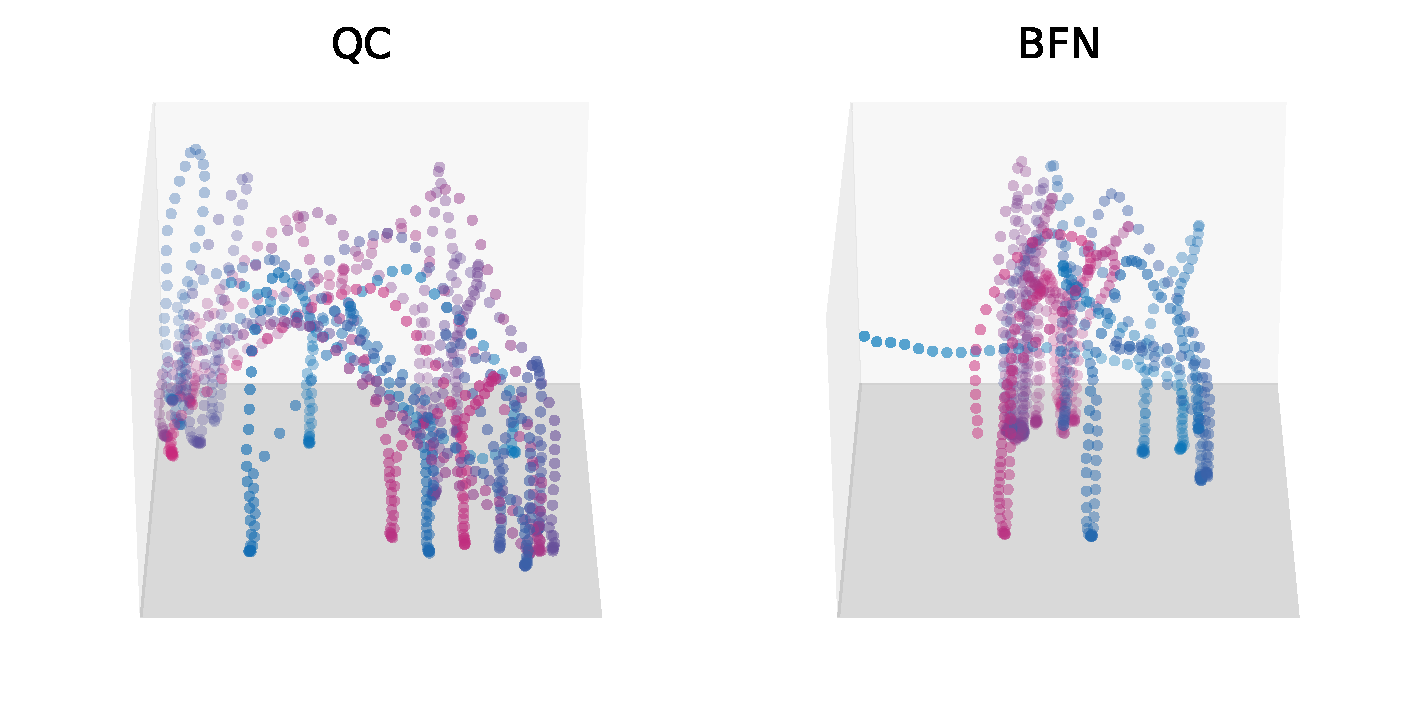
\includegraphics[width=0.32\linewidth]{figures/viz/traj_viz_comb_0_simplified.pdf}
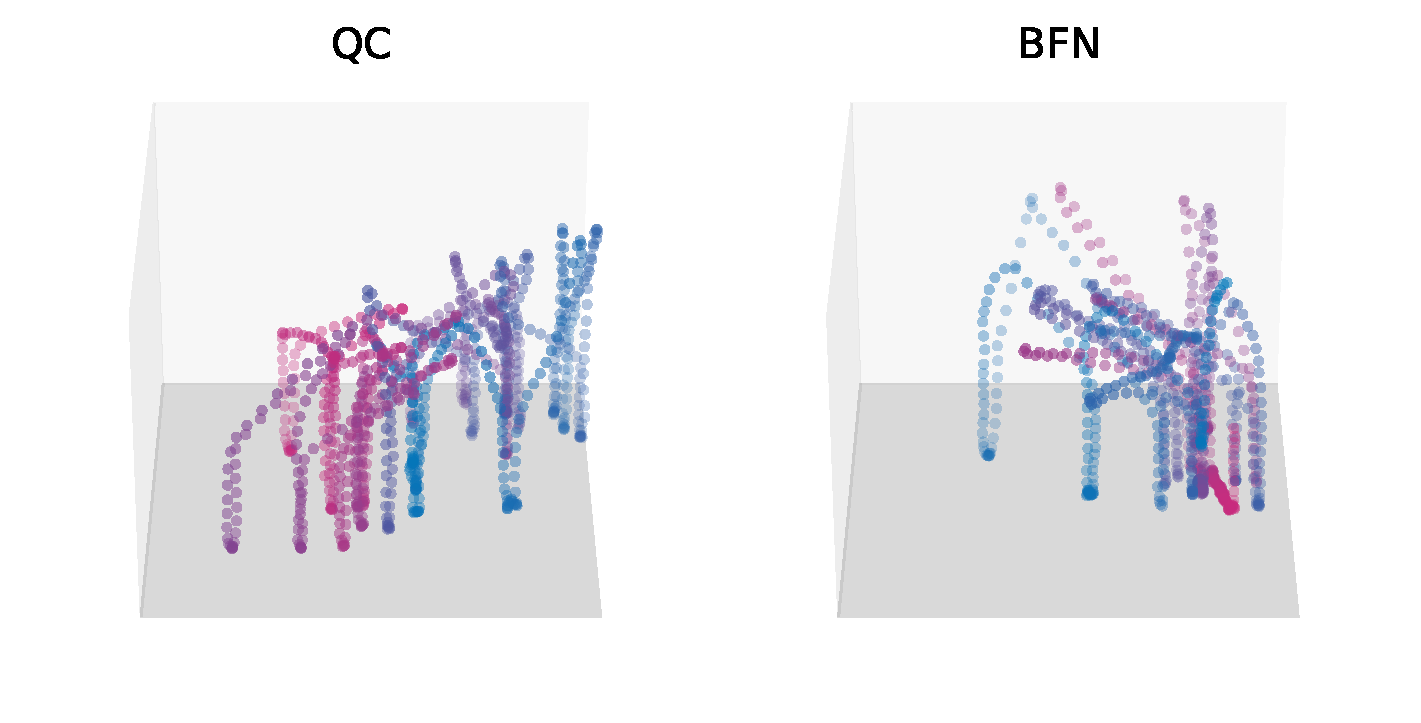
\includegraphics[width=0.32\linewidth]{figures/viz/traj_viz_comb_1_simplified.pdf}
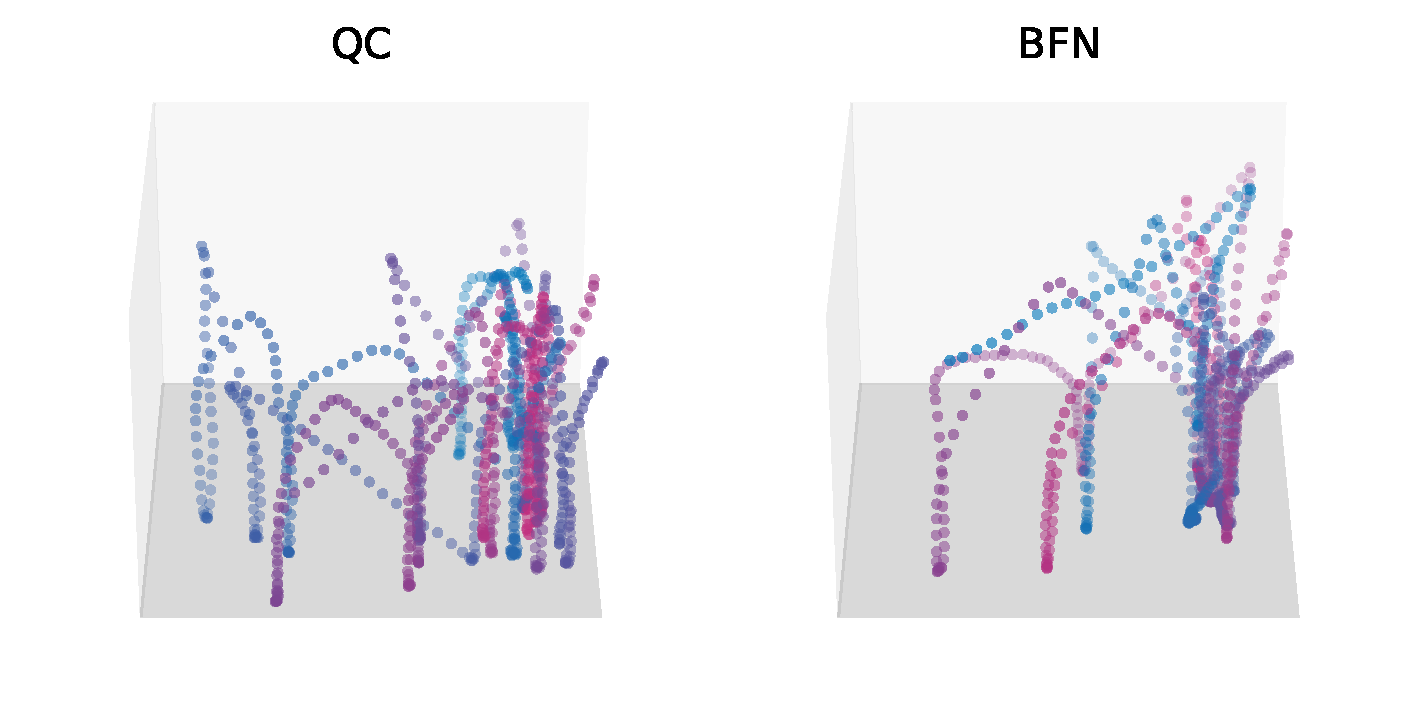
\includegraphics[width=0.32\linewidth]{figures/viz/traj_viz_comb_2_simplified.pdf}
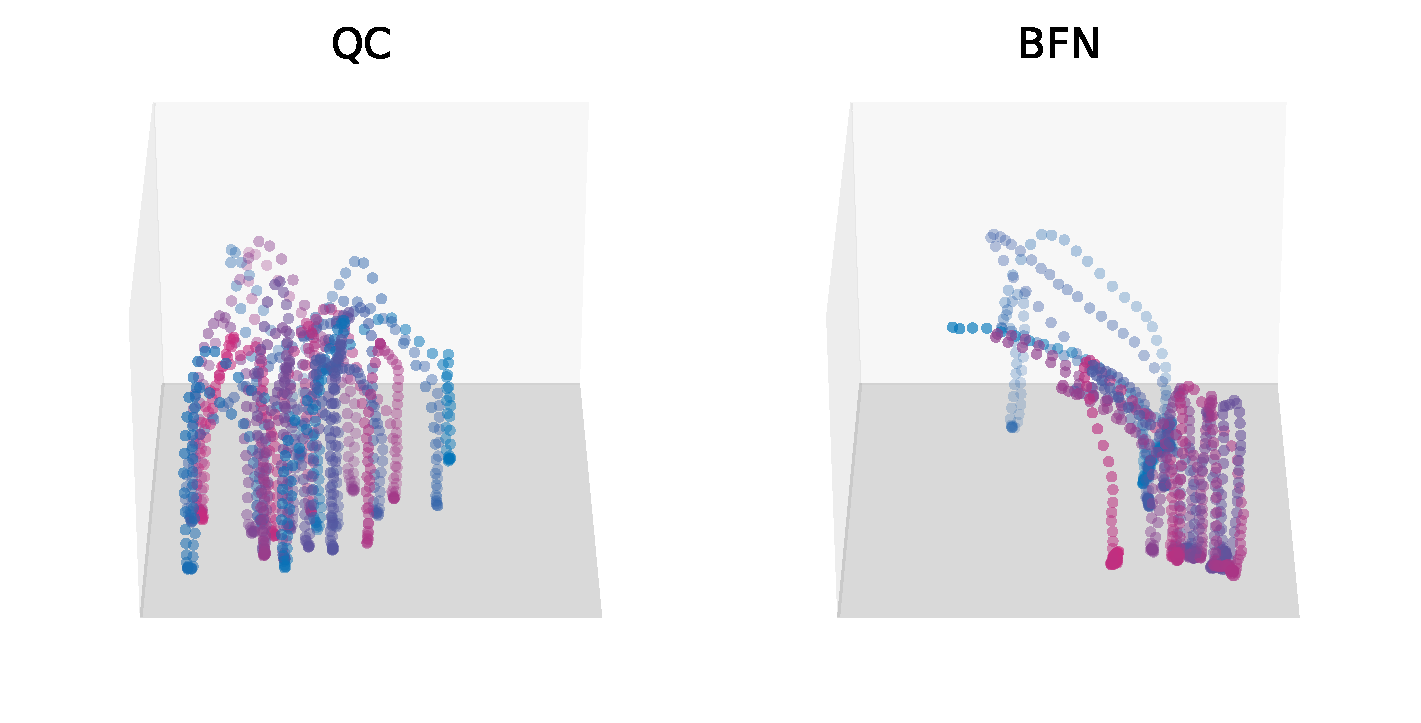
\includegraphics[width=0.32\linewidth]{figures/viz/traj_viz_comb_3_simplified.pdf}
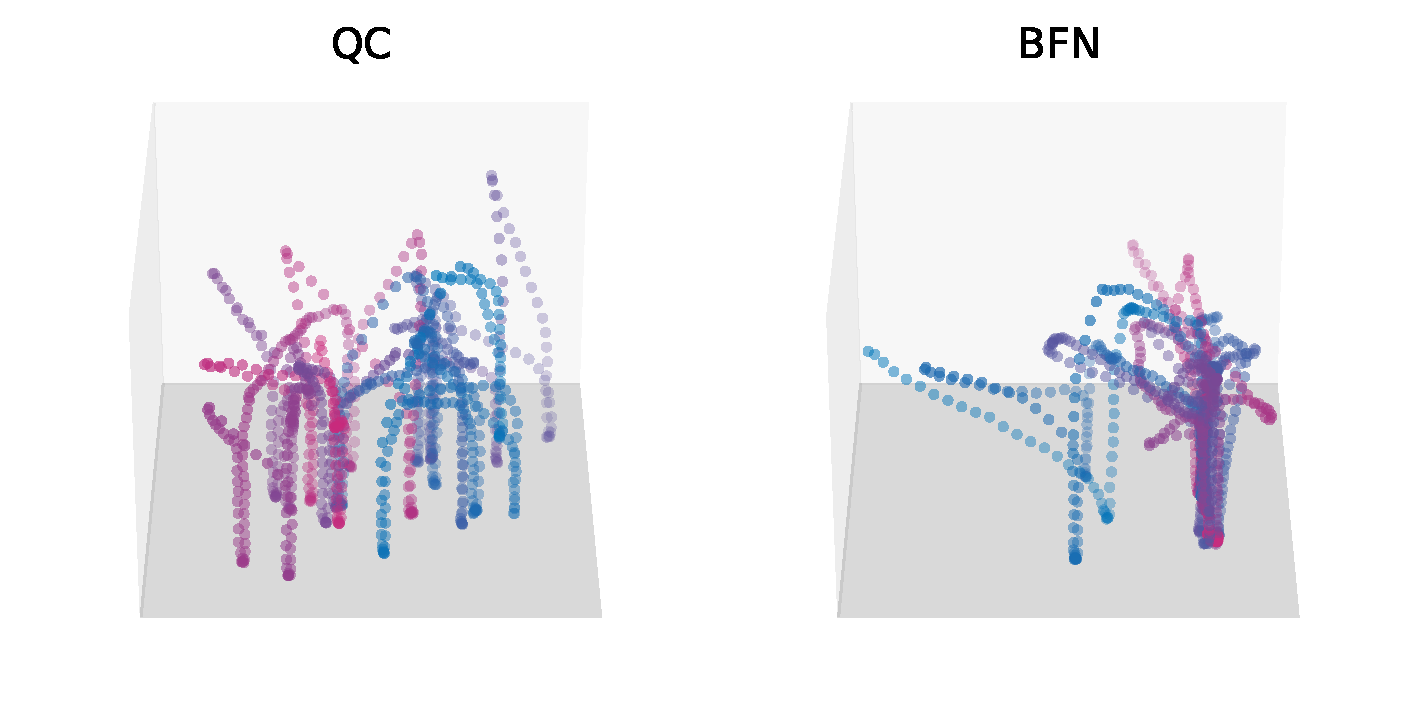
\includegraphics[width=0.32\linewidth]{figures/viz/traj_viz_comb_4_simplified.pdf}
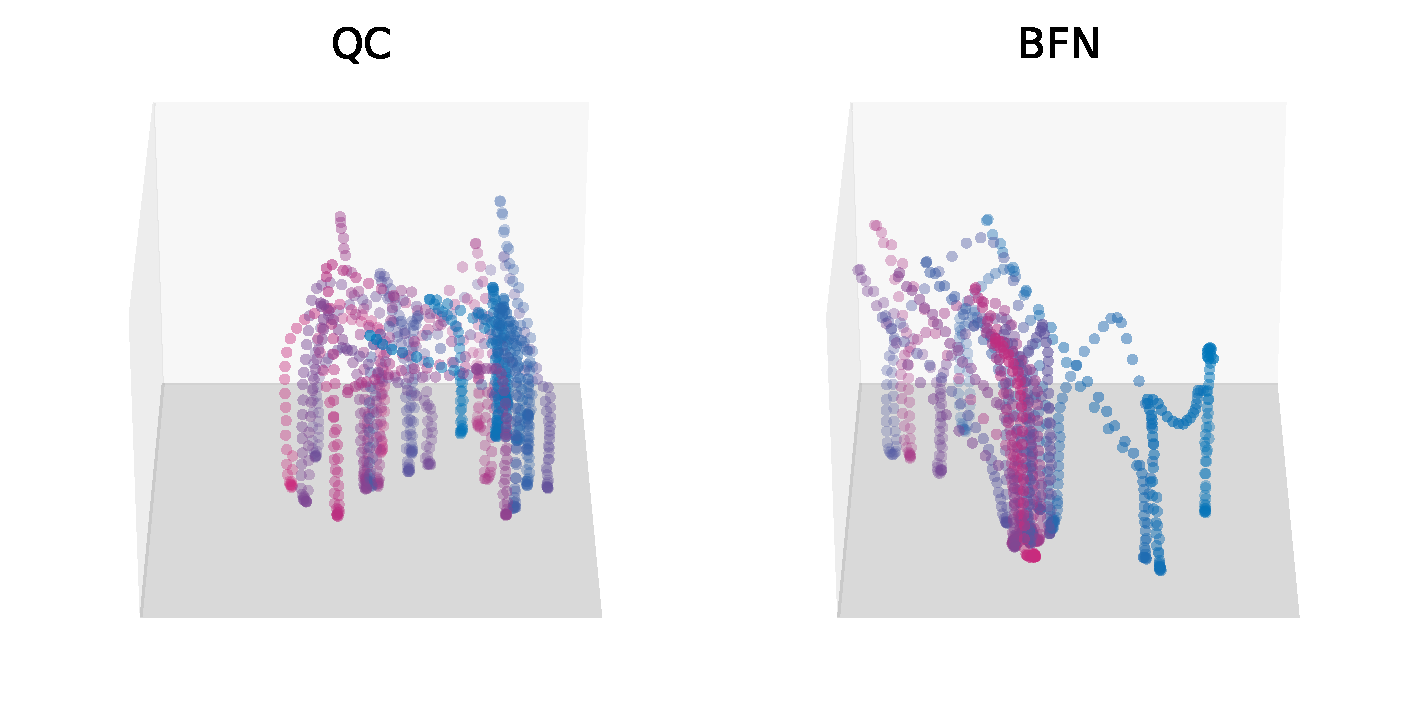
\includegraphics[width=0.32\linewidth]{figures/viz/traj_viz_comb_5_simplified.pdf}
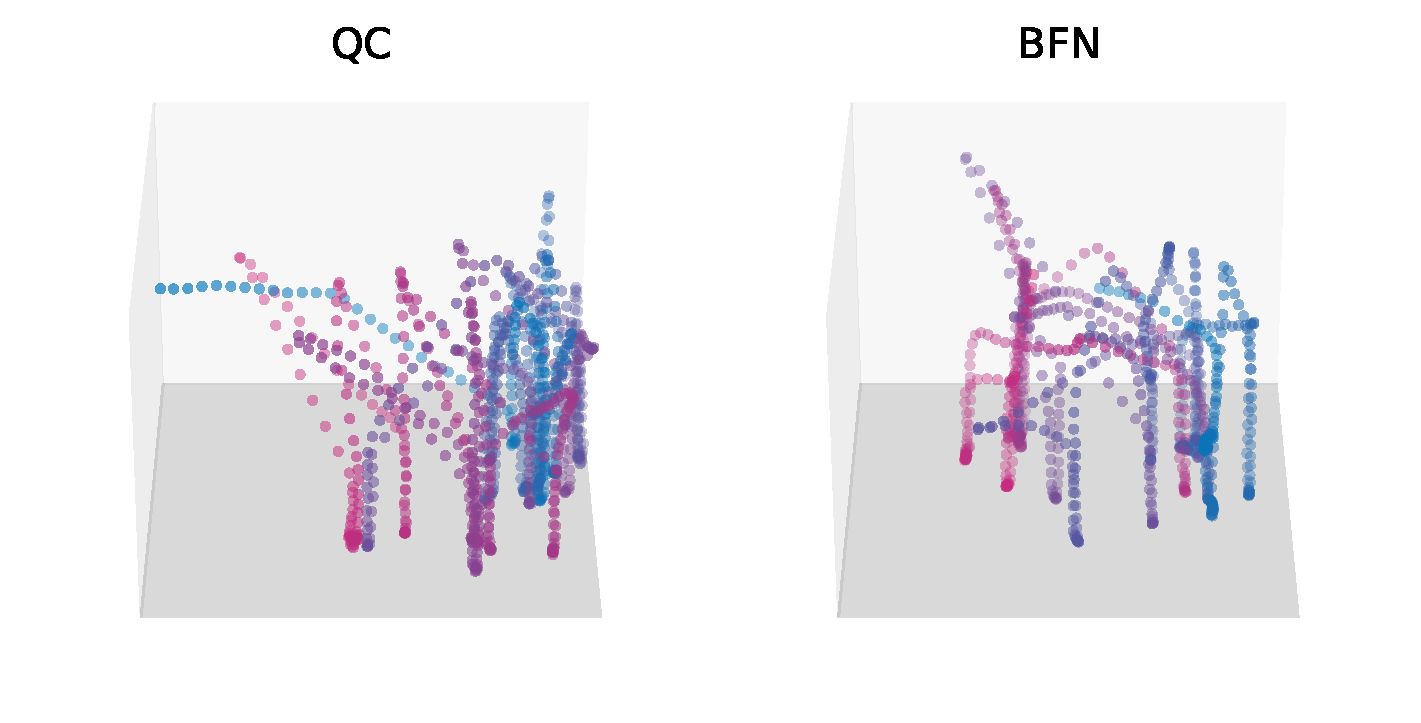
\includegraphics[width=0.32\linewidth]{figures/viz/traj_viz_comb_6_simplified.pdf}
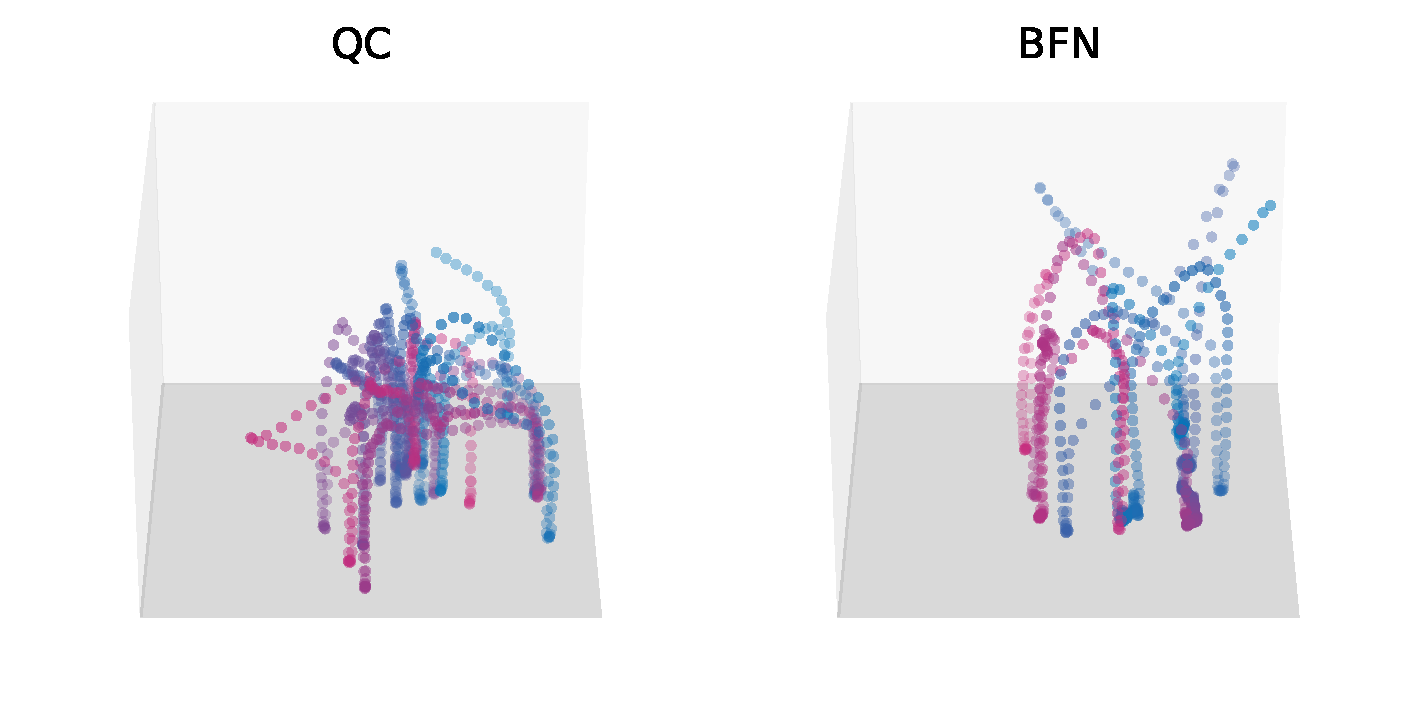
\includegraphics[width=0.32\linewidth]{figures/viz/traj_viz_comb_7_simplified.pdf}
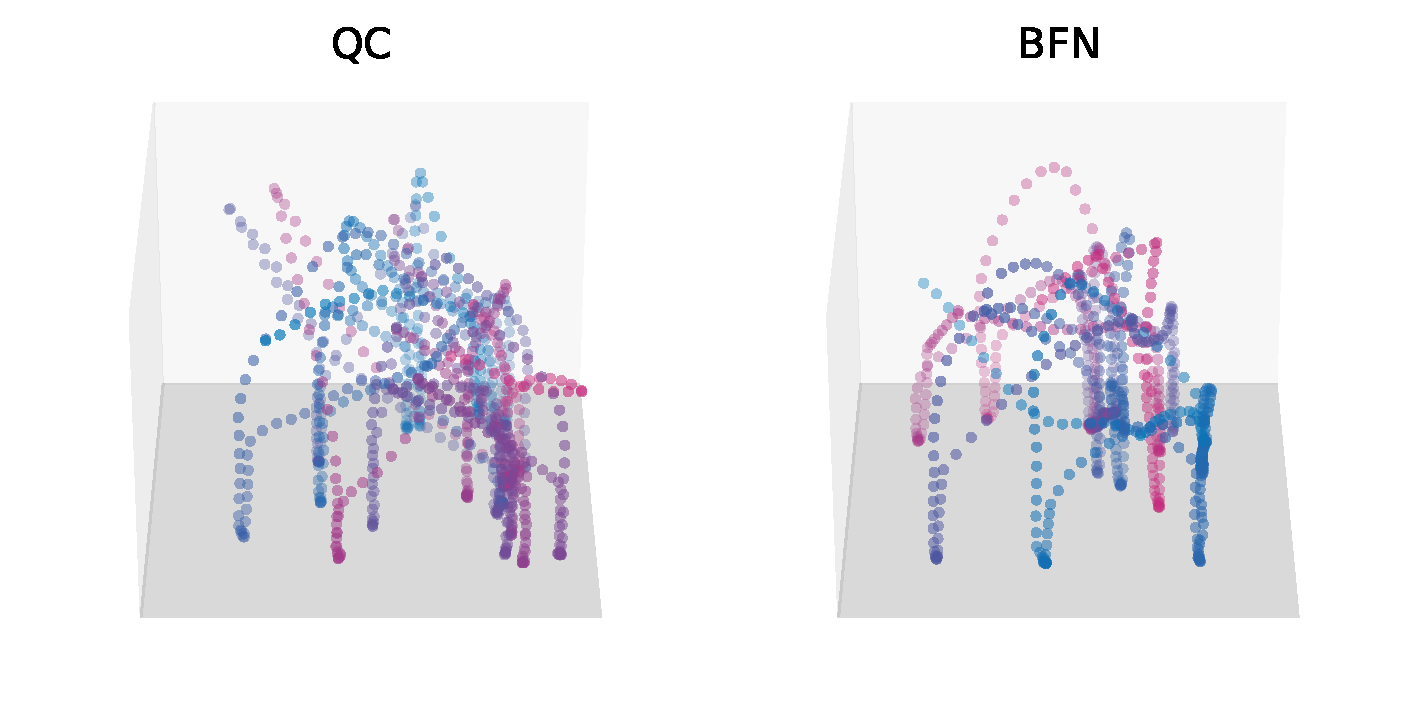
\includegraphics[width=0.32\linewidth]{figures/viz/traj_viz_comb_8_simplified.pdf}
\caption{\textbf{End-effector trajectory early in the training.} Each subplot above shows the trajectory for a consecutive of 1000 time steps. We include up to Step 9000.}
\label{fig:traj-viz-early}
\end{figure}


\begin{figure}[H]
    \centering
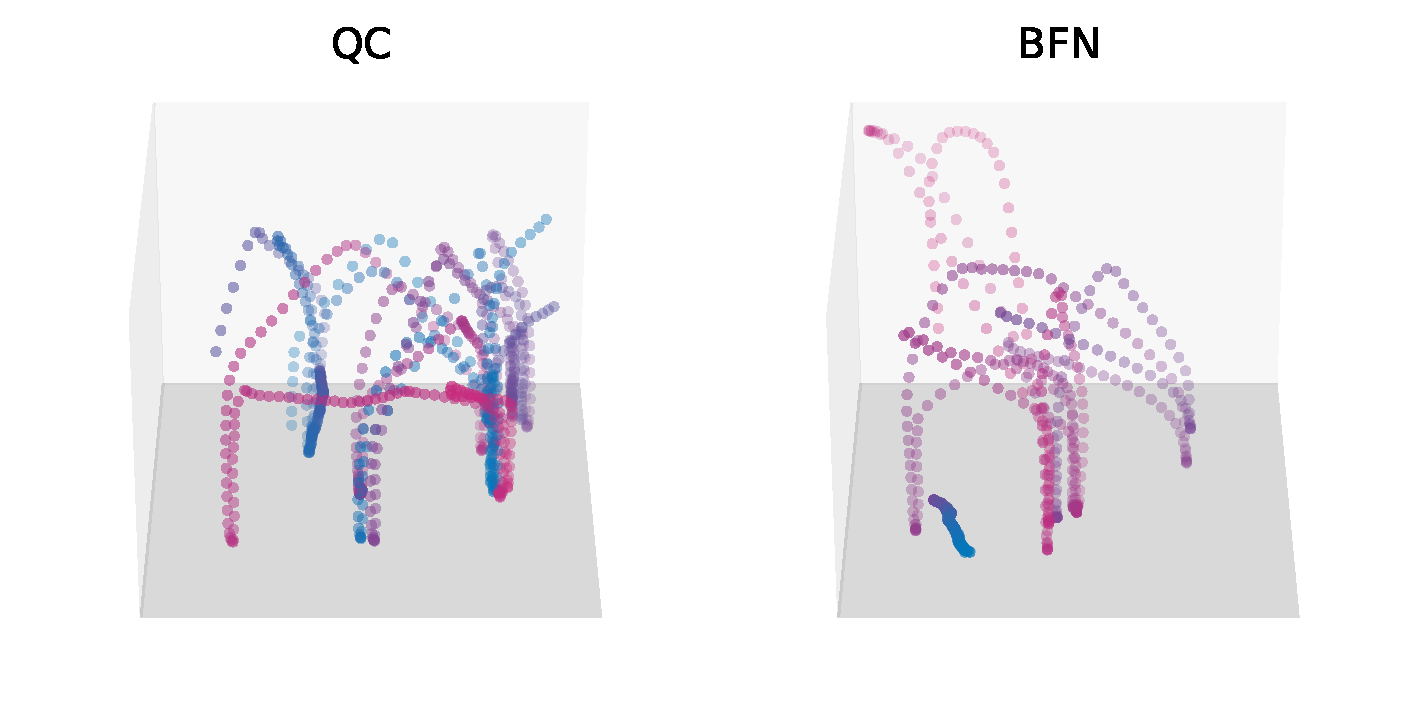
\includegraphics[width=0.32\linewidth]{figures/viz/traj_viz_comb_900_simplified.pdf}
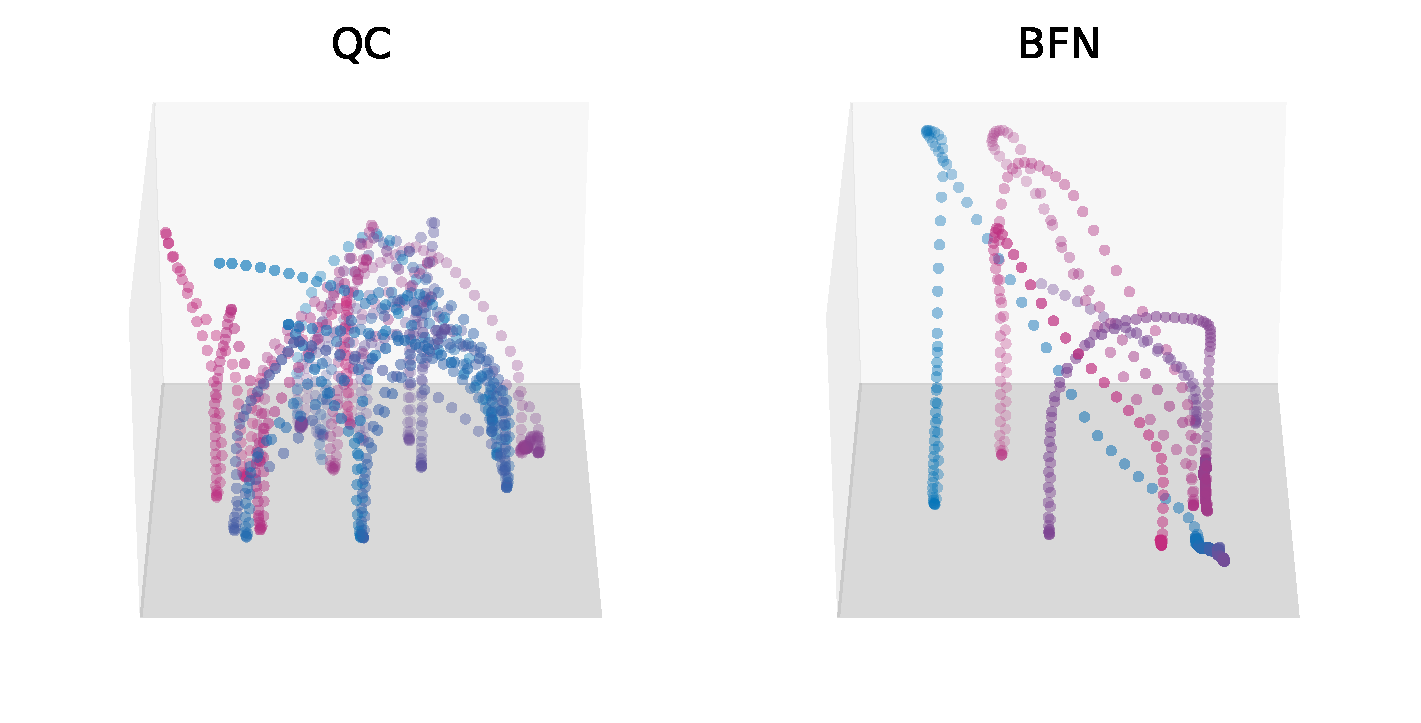
\includegraphics[width=0.32\linewidth]{figures/viz/traj_viz_comb_901_simplified.pdf}
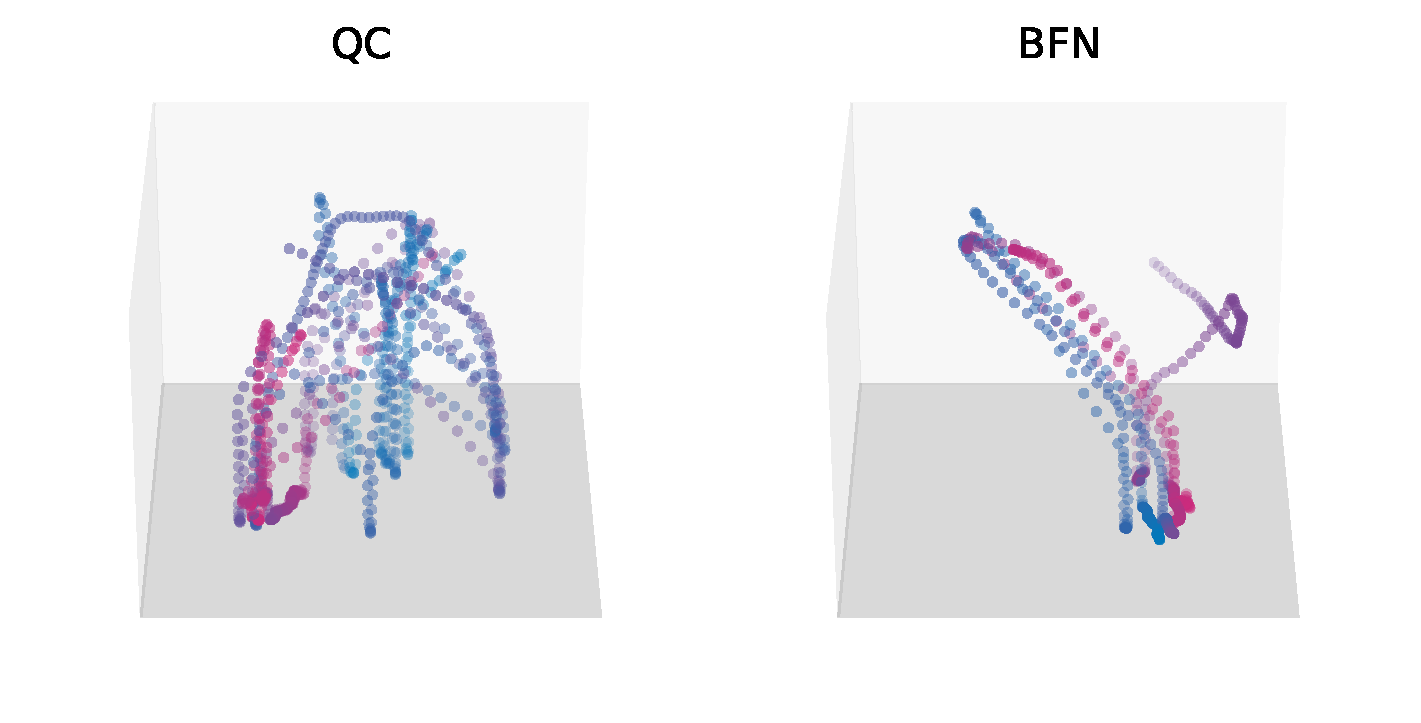
\includegraphics[width=0.32\linewidth]{figures/viz/traj_viz_comb_902_simplified.pdf}
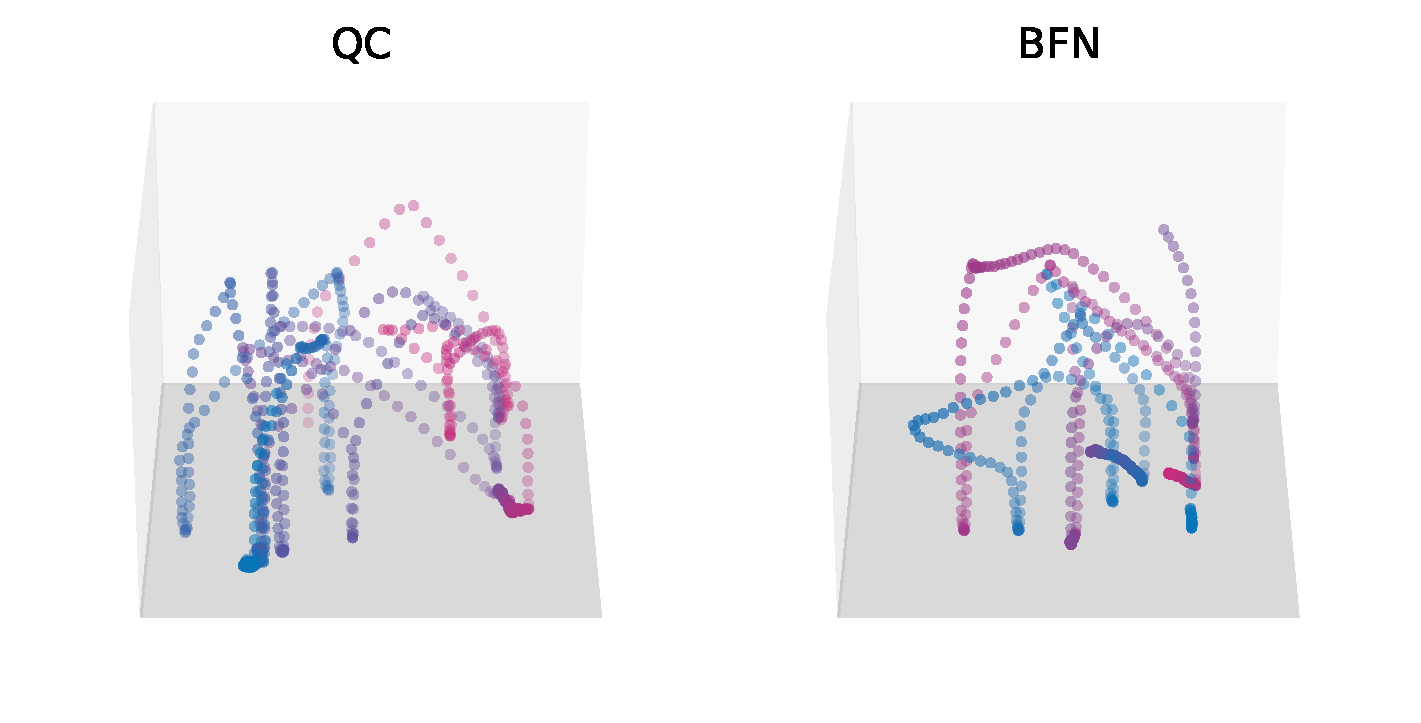
\includegraphics[width=0.32\linewidth]{figures/viz/traj_viz_comb_903_simplified.pdf}
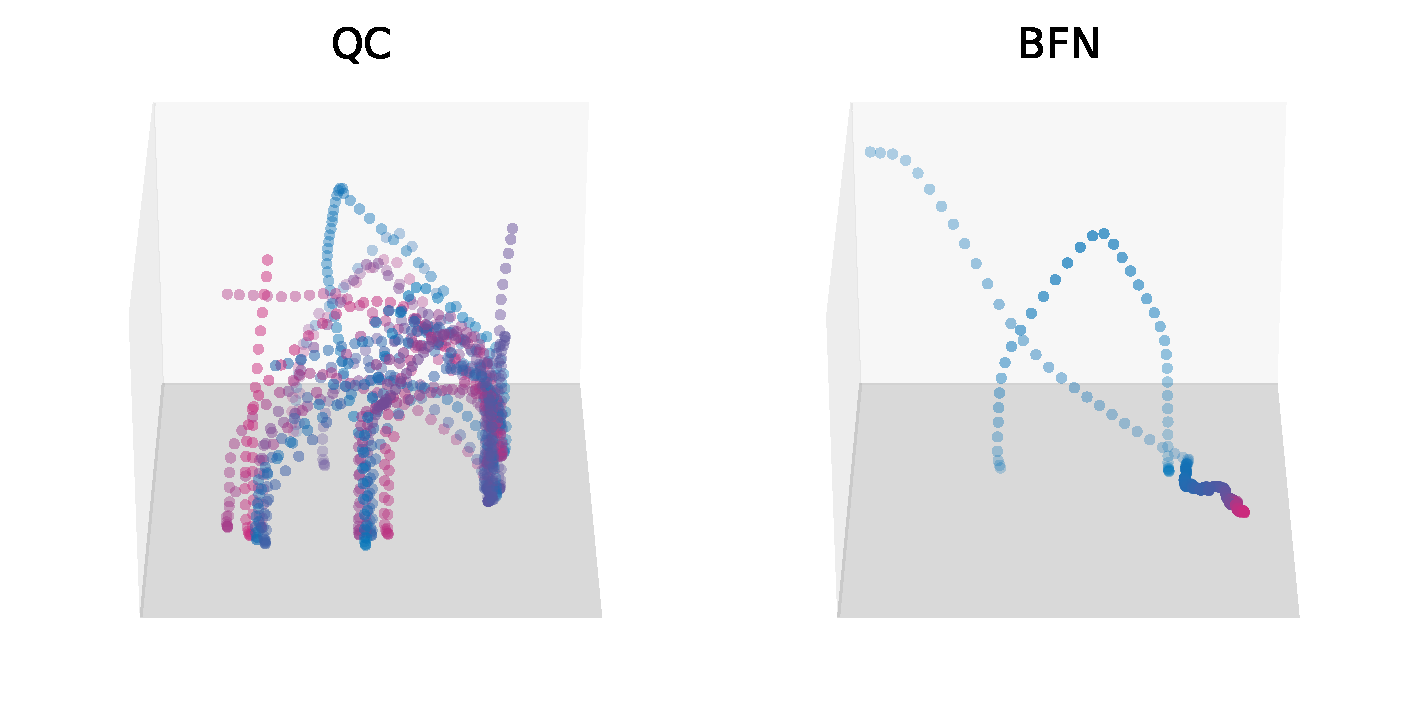
\includegraphics[width=0.32\linewidth]{figures/viz/traj_viz_comb_904_simplified.pdf}
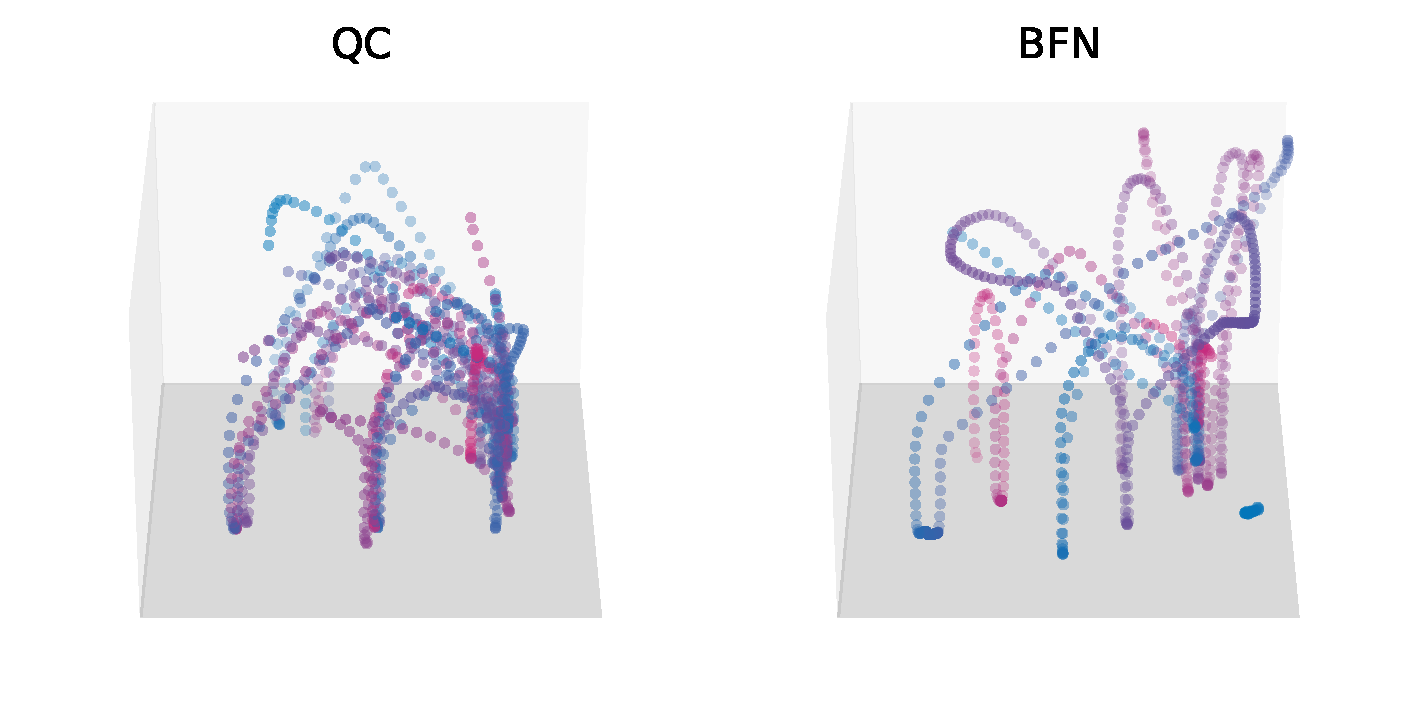
\includegraphics[width=0.32\linewidth]{figures/viz/traj_viz_comb_905_simplified.pdf}
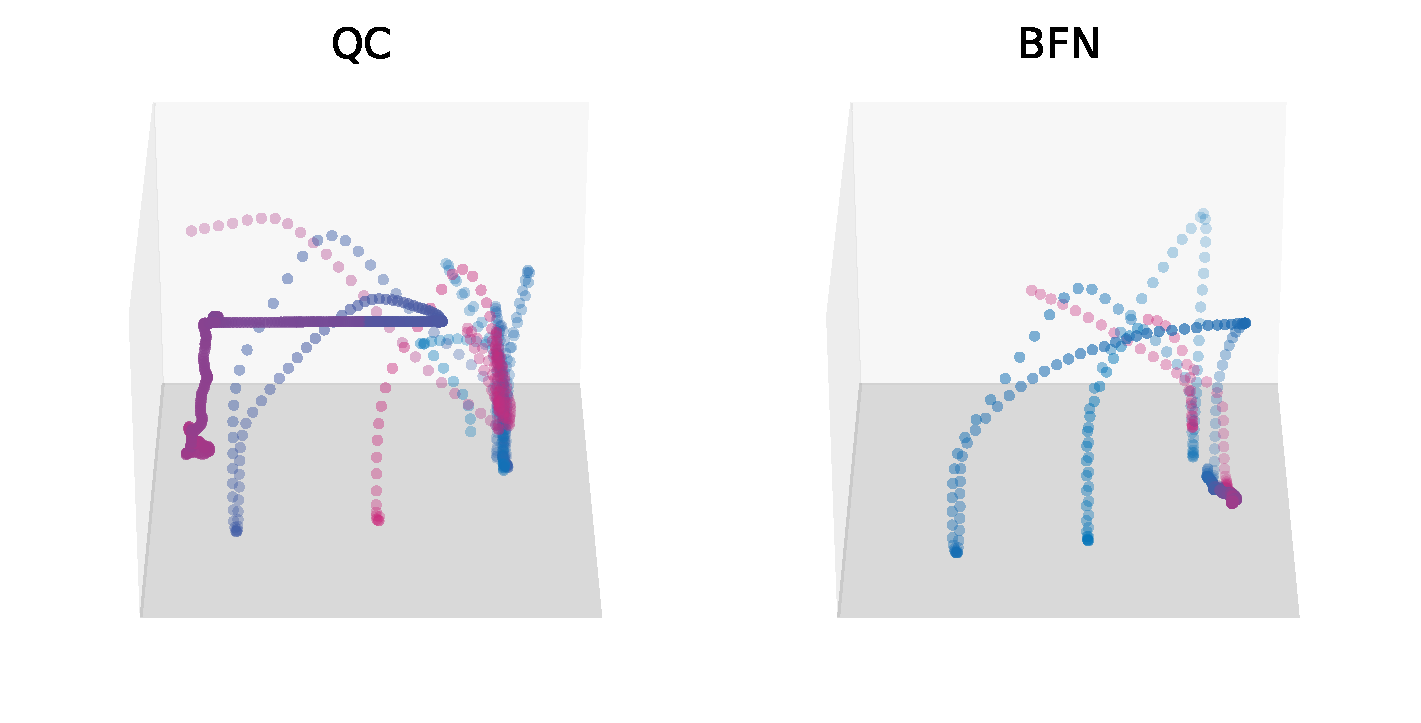
\includegraphics[width=0.32\linewidth]{figures/viz/traj_viz_comb_906_simplified.pdf}
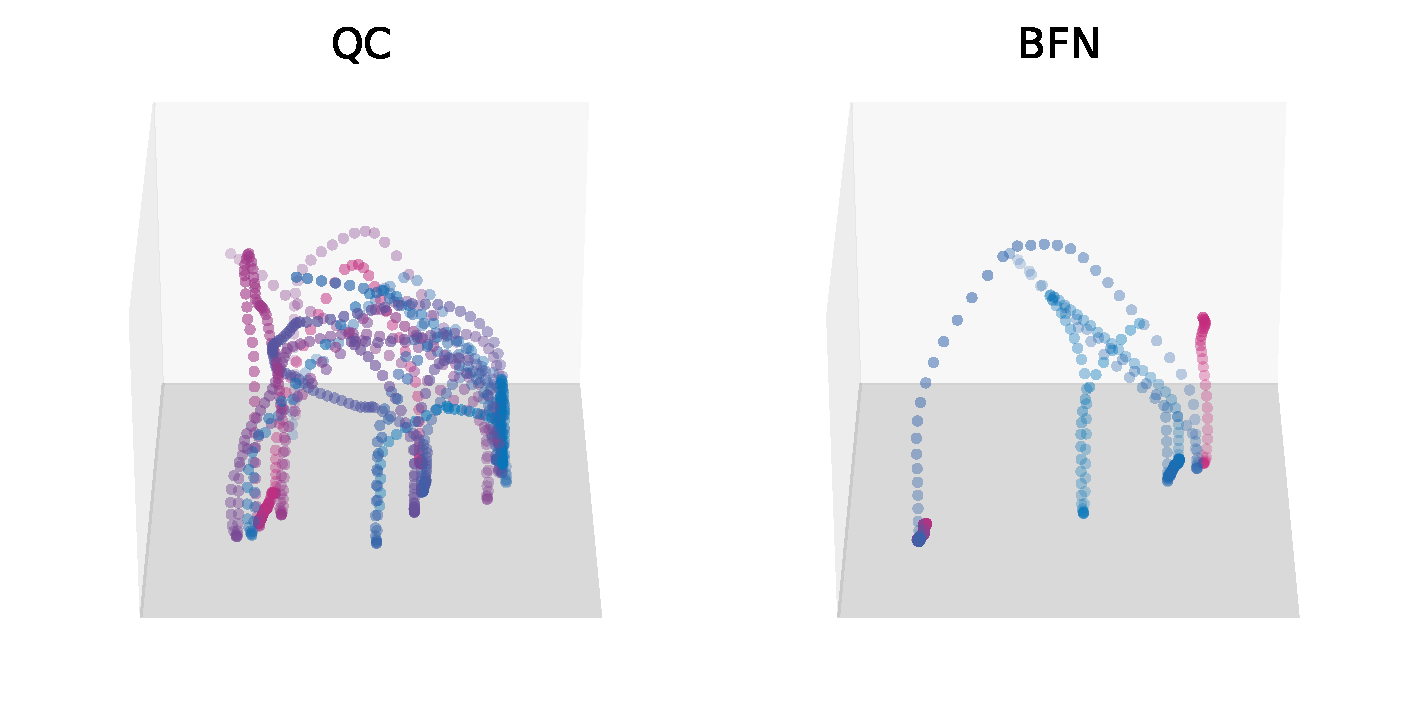
\includegraphics[width=0.32\linewidth]{figures/viz/traj_viz_comb_907_simplified.pdf}
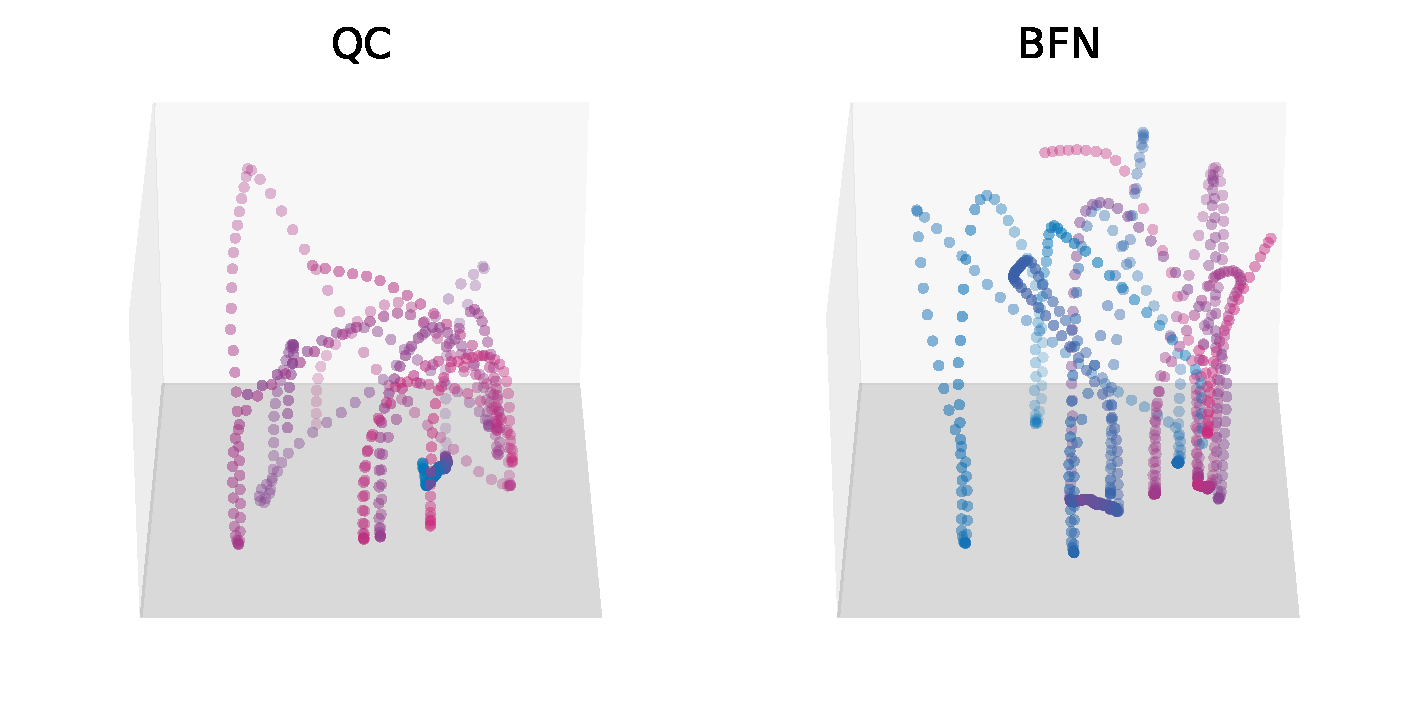
\includegraphics[width=0.32\linewidth]{figures/viz/traj_viz_comb_908_simplified.pdf}
\caption{\textbf{End-effector trajectory visualization late in the training.} Each subplot above shows the trajectory for a consecutive of 1000 time steps. We include the trajectories from Step 900000 to Step 99000.}
\label{fig:traj-viz-late}
\end{figure}

\subsection{OGBench results by individual task}

\textbf{Main results by task.} The following plot (\cref{fig:main-all-individual} shows the performance breakdown for \cref{fig:main}.
\begin{figure}[H]
    \centering
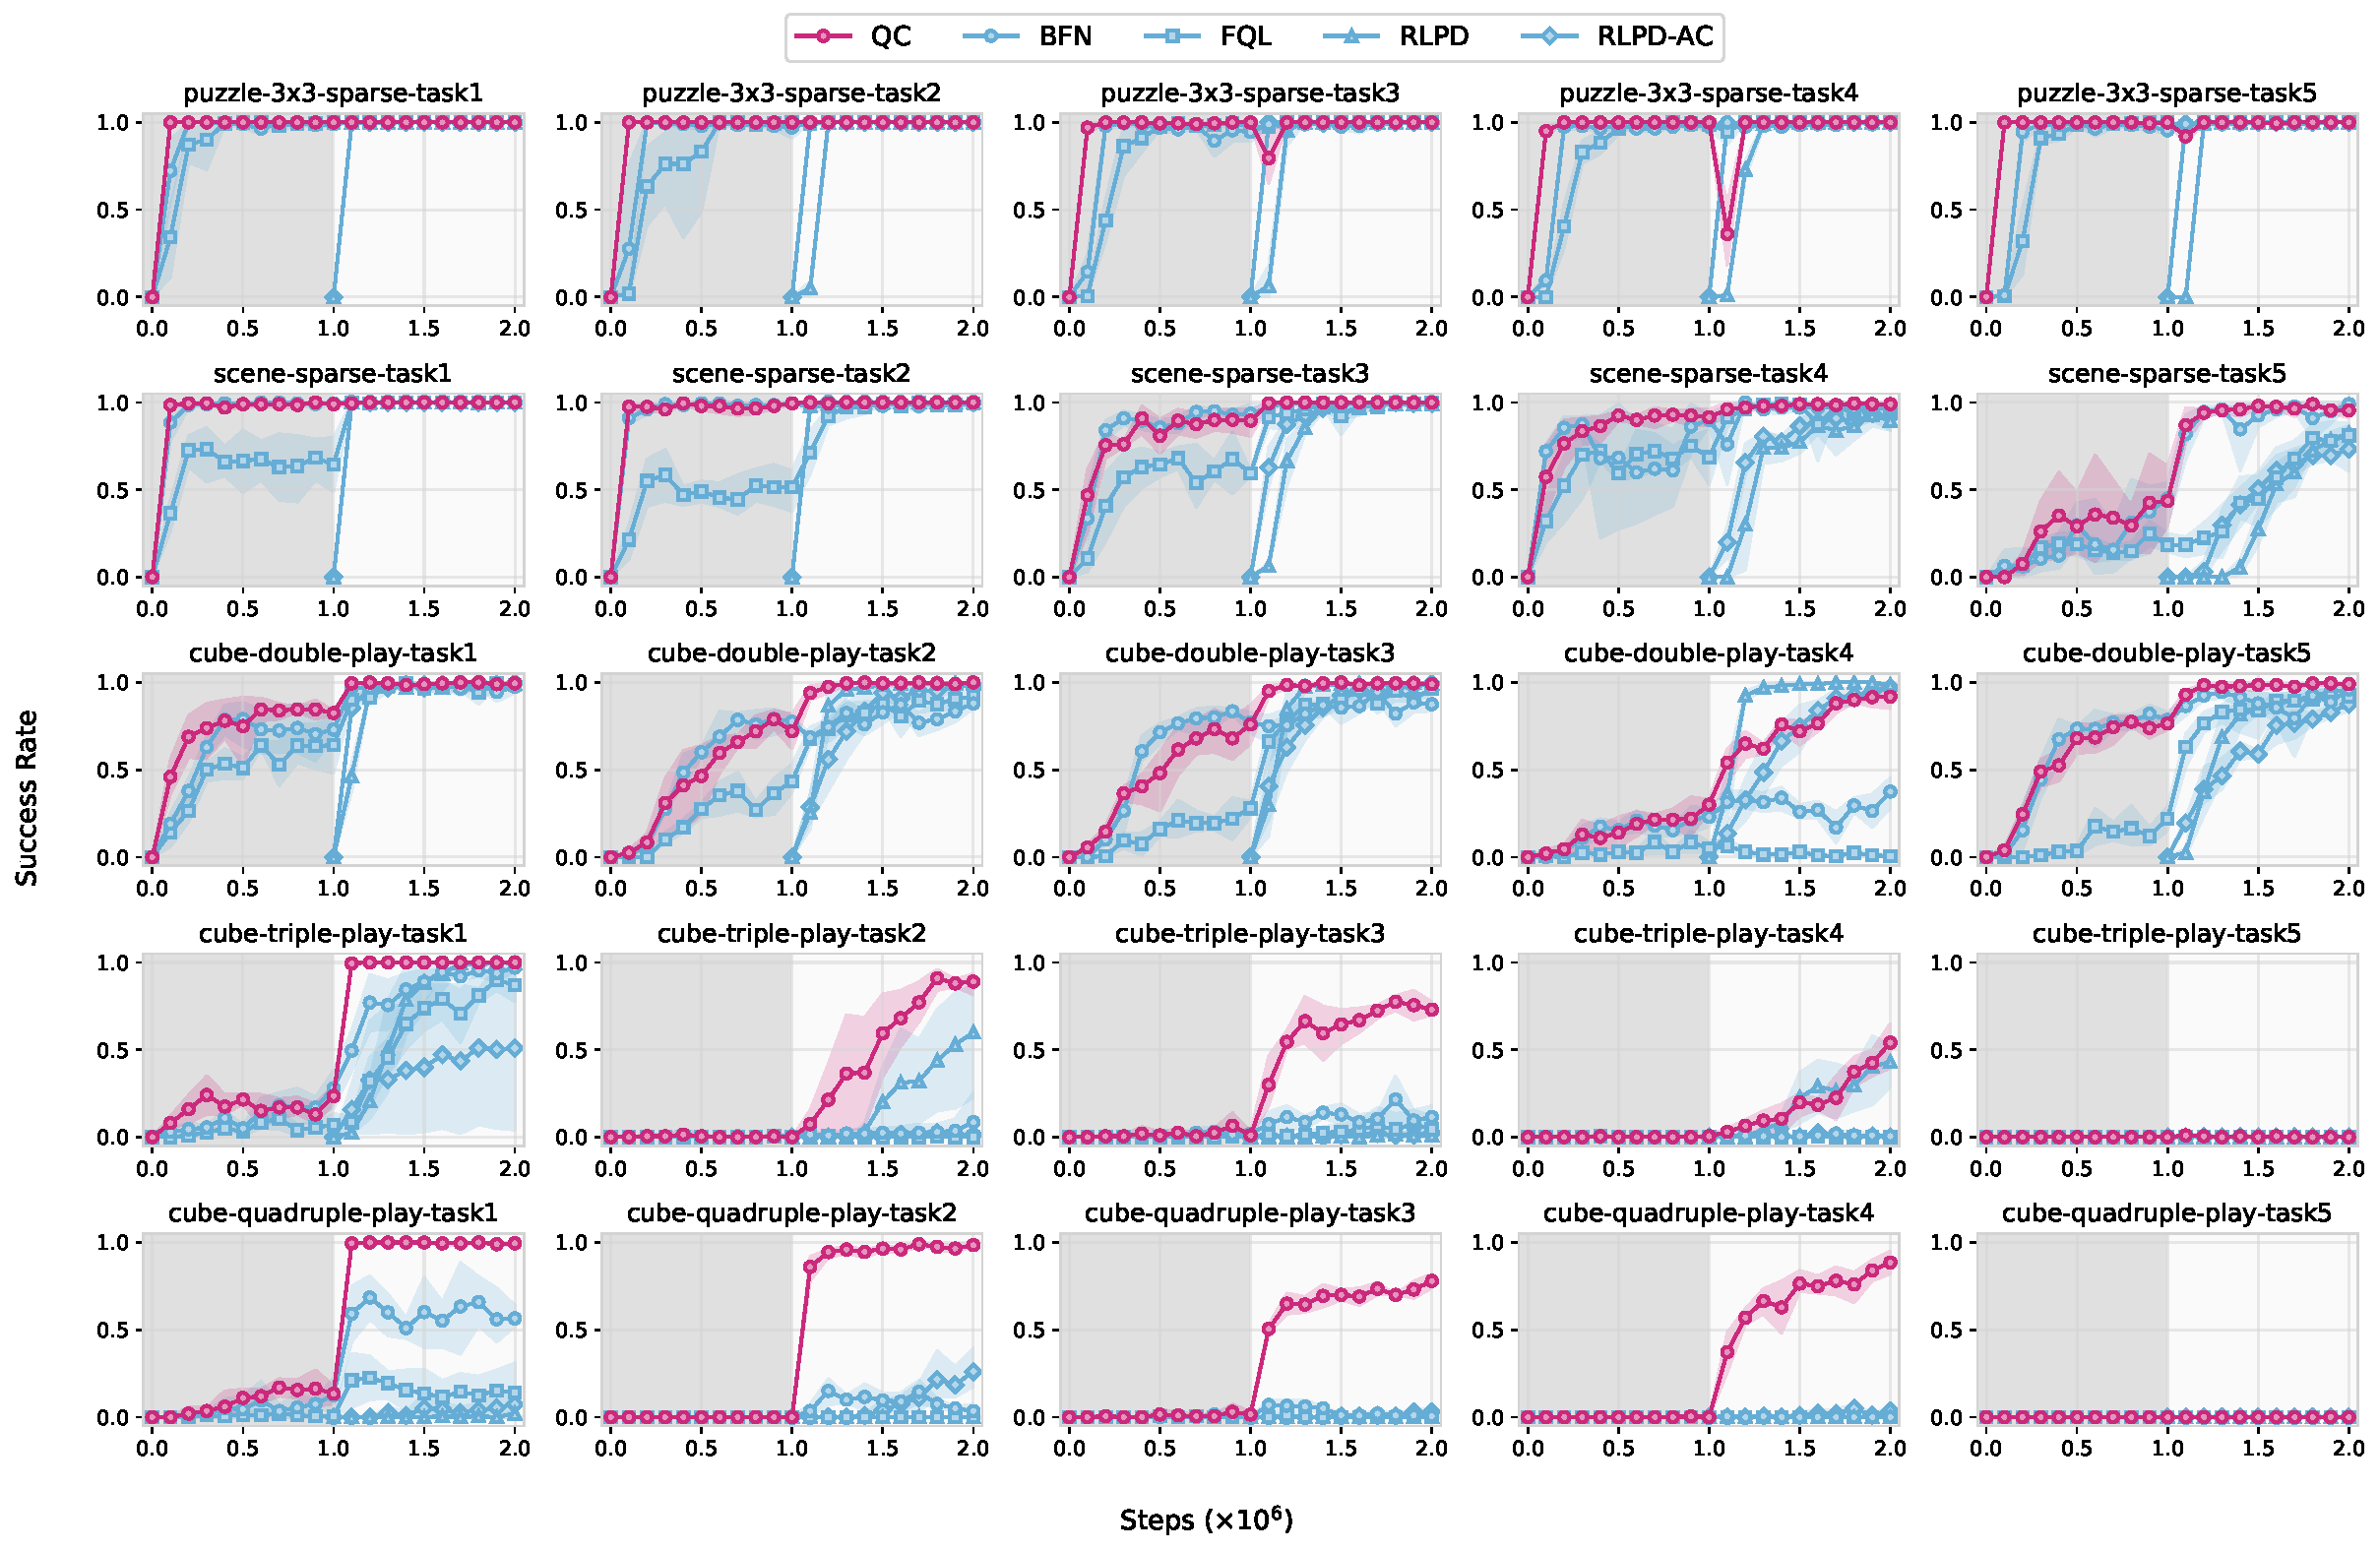
\includegraphics[width=\linewidth]{figures/main-all-individual-ablation.pdf}
    \caption{\textbf{Full OGBench results by task.} For each method on each task, we use 4 seeds.}
    \label{fig:main-all-individual}
\end{figure}


\textbf{Ablation results by task.} The following plot (\cref{fig:ablation-all-individual}) shows the performance breakdown for \cref{fig:ablation}.
\begin{figure}[H]
    \centering
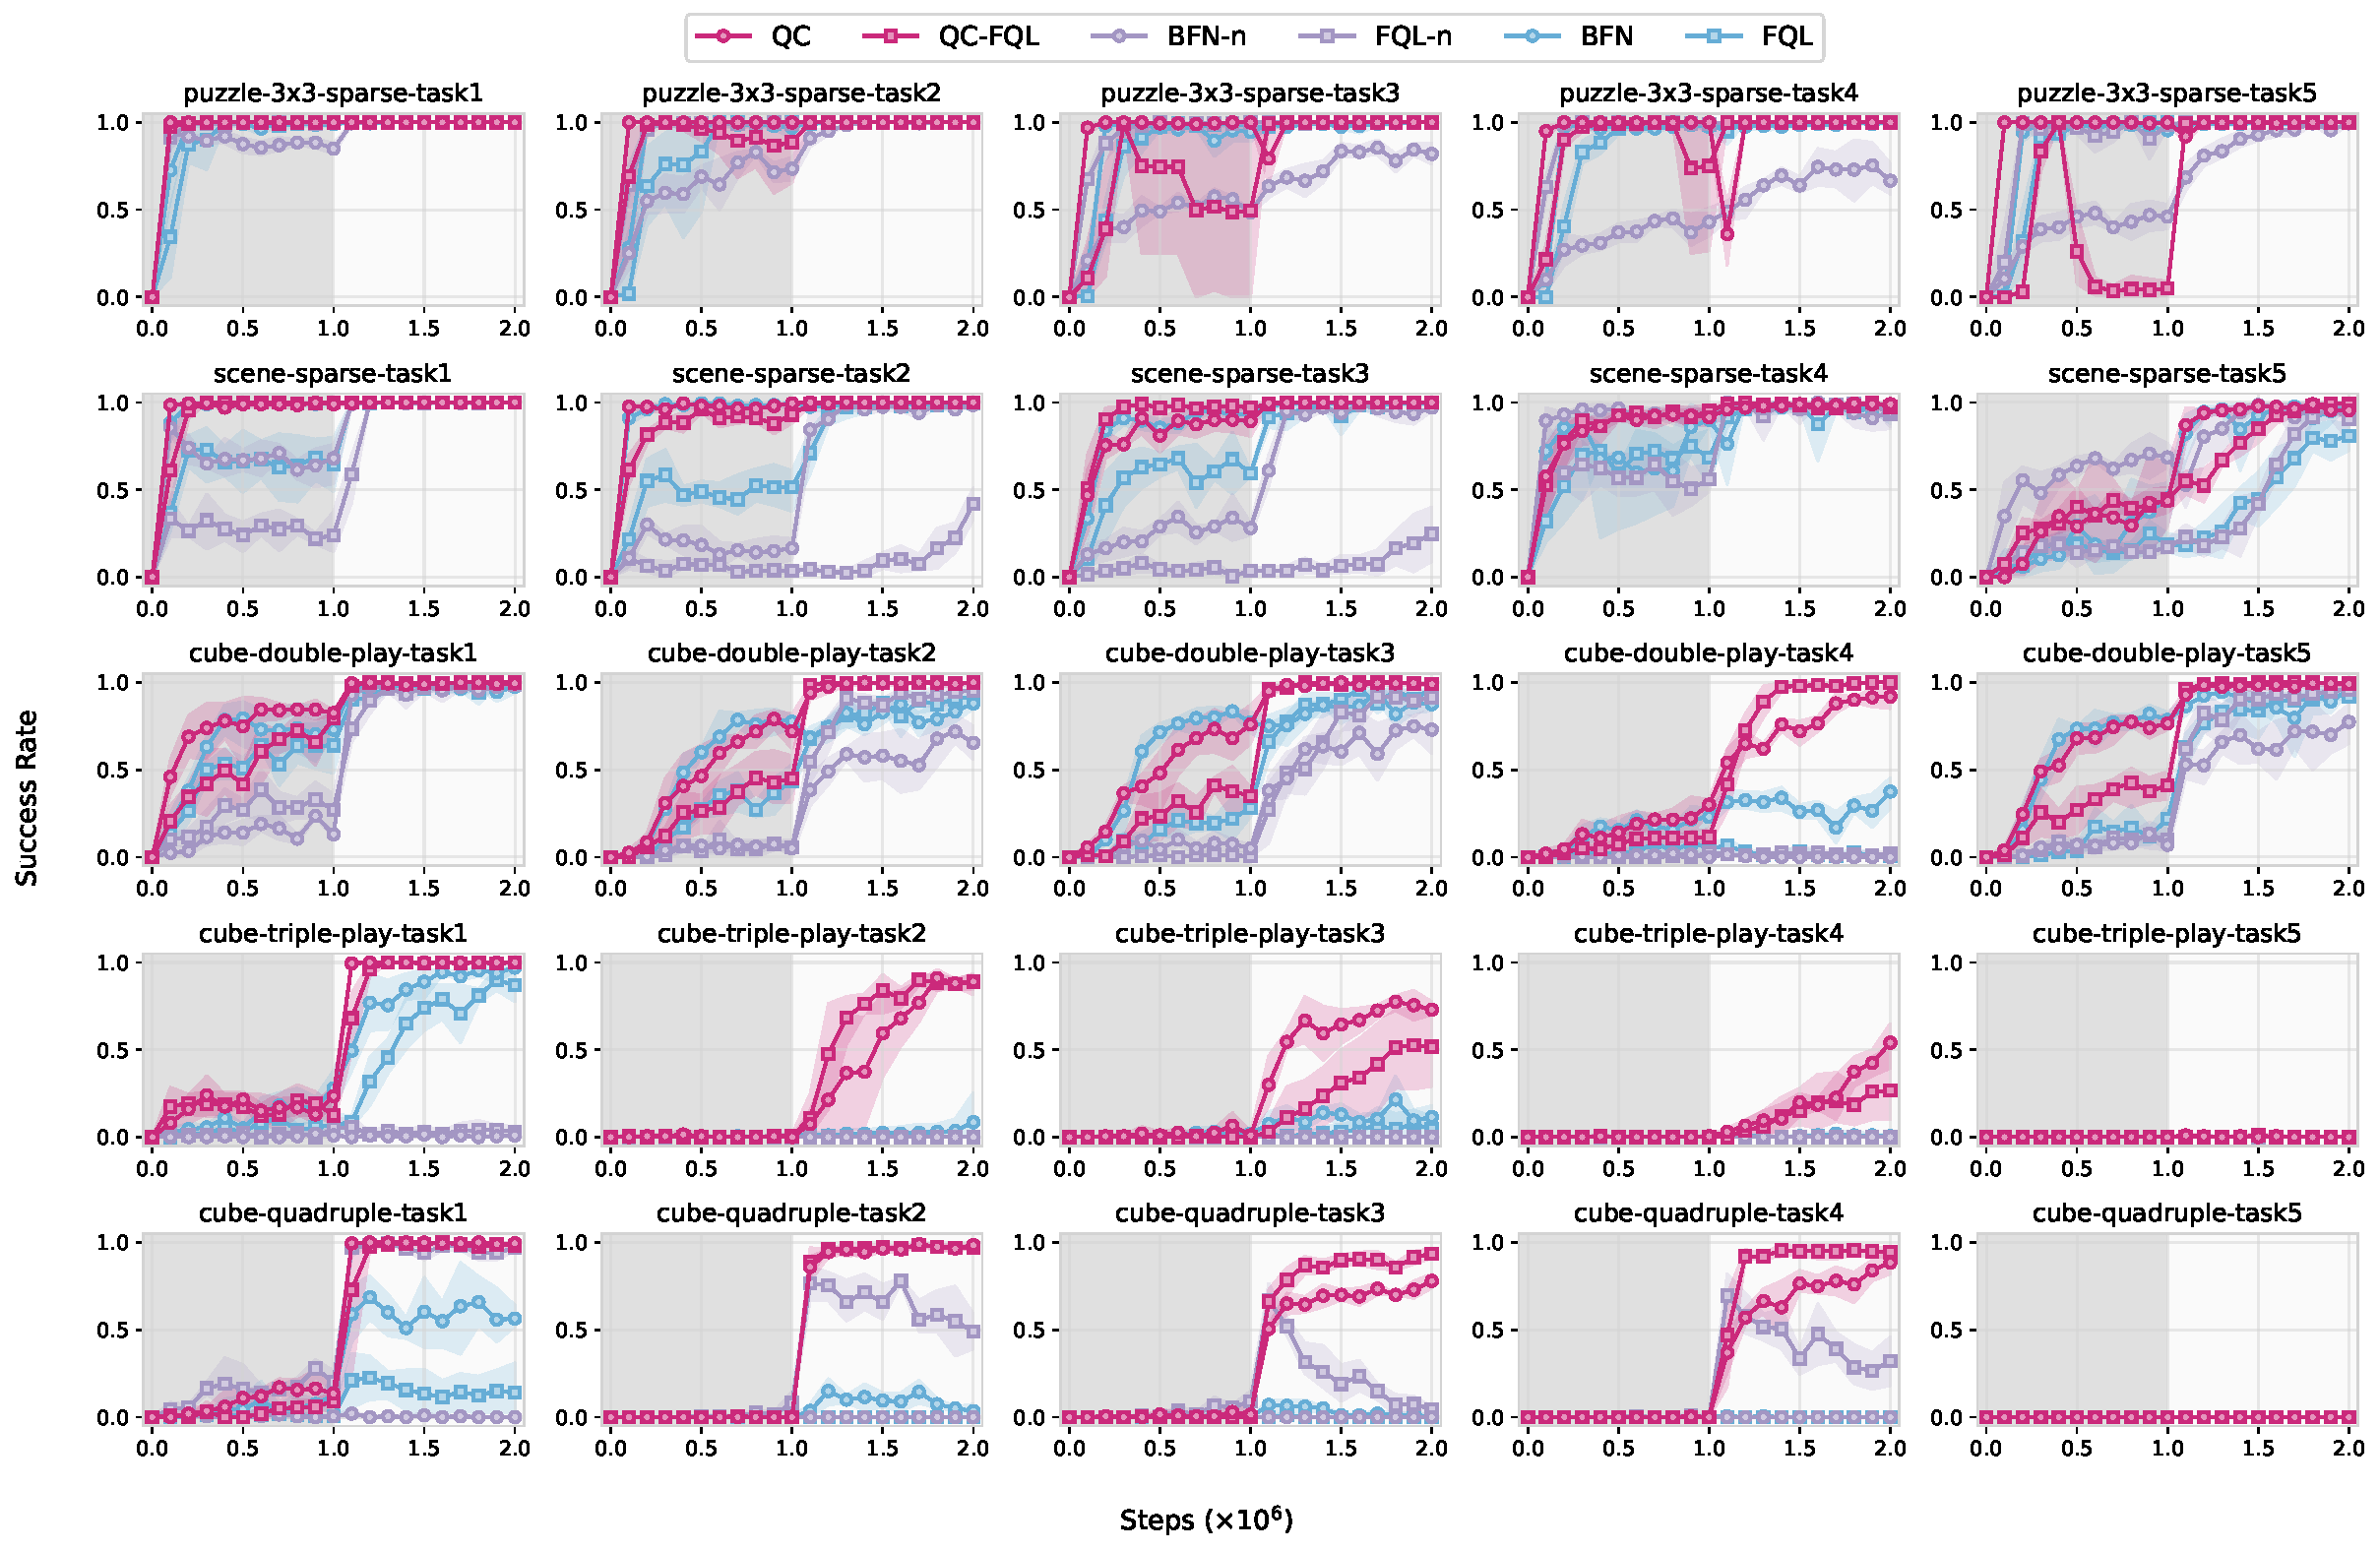
\includegraphics[width=\linewidth]{figures/main-all-individual.pdf}
    \caption{\textbf{Full OGBench results by task.} For each method on each task, we use 4 seeds.}
    \label{fig:ablation-all-individual}
\end{figure}


\textbf{Q-chunking with Gausian policies.}
The following plot shows the performance breakdown for \cref{fig:rlpd-all}. In addition, we include a new method for comparison, \hourpurple{QC-RLPD}, where we add a behavior cloning loss to \hourblue{RLPD-AC} (\hourblue{RLPD} with action chunking).
\begin{figure}[H]
    \centering
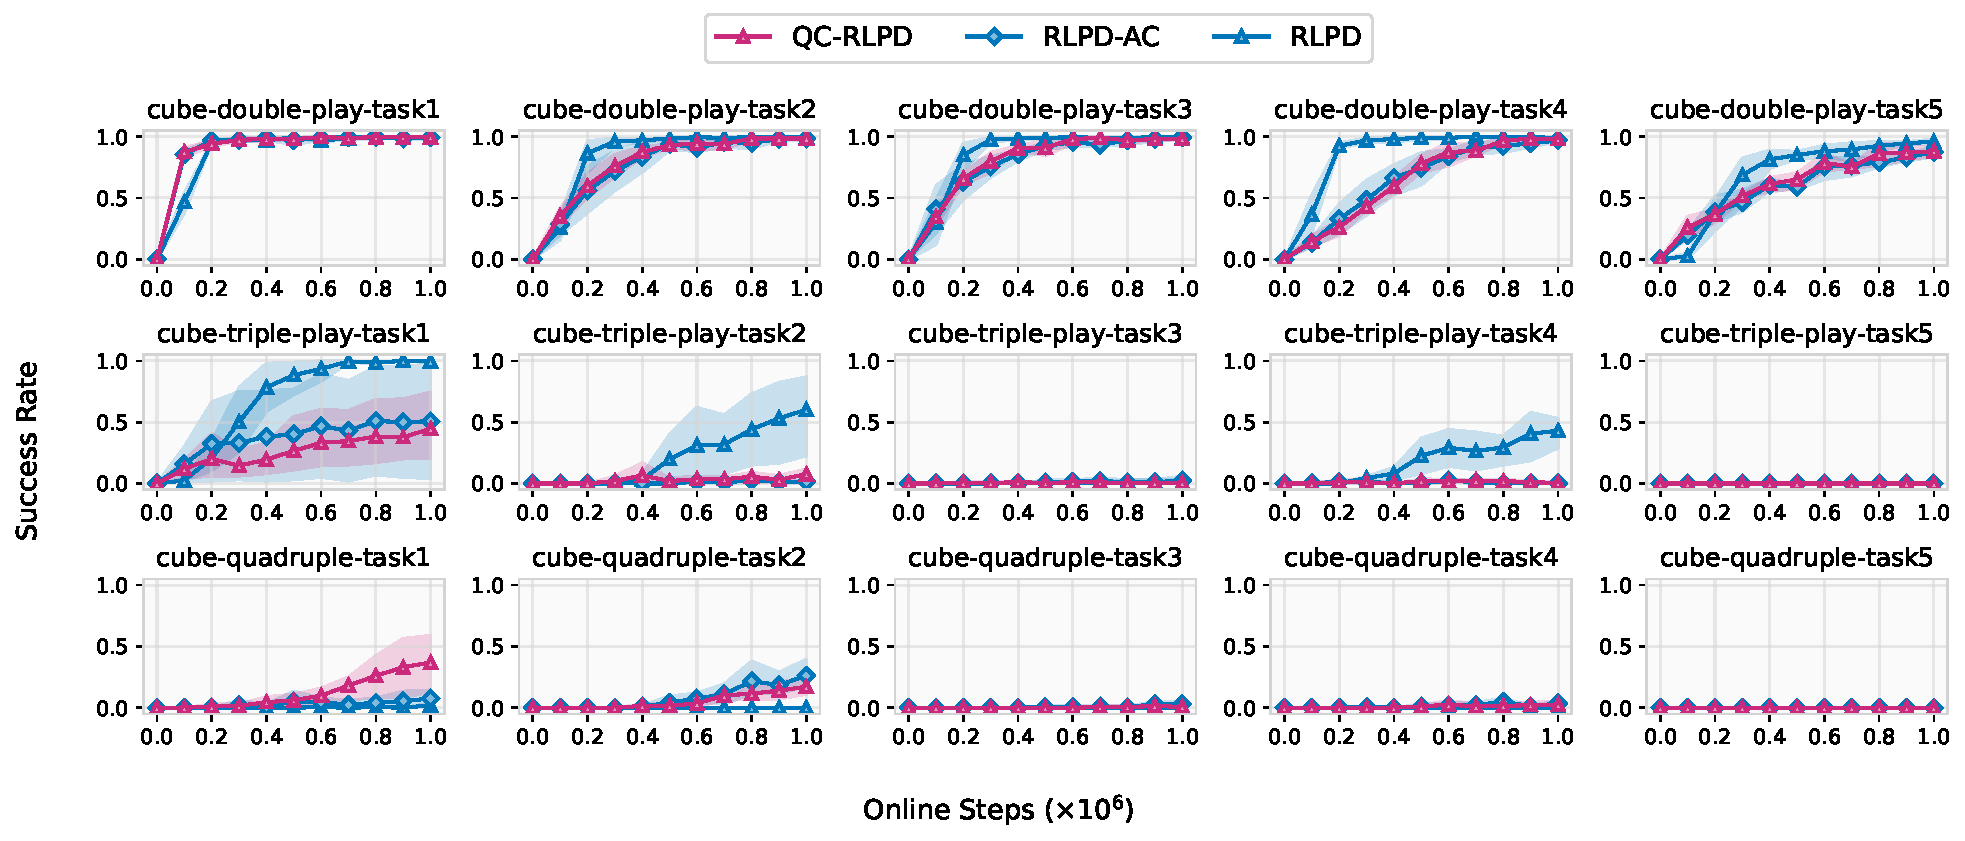
\includegraphics[width=\linewidth]{figures/rlpd-qc-all-individual.pdf}
    \caption{\textbf{Full \hourblue{RLPD} results by task.} For each method on each task, we use 4 seeds. \hourpurple{QC-RLPD} is \hourblue{RLPD-AC} (\hourblue{RLPD} on the temporally extended action space) where we additionally add a fixed behavior cloning coefficient of $0.01$.}
    \label{fig:rlpd-all-ind}
\end{figure}

\subsection{Robomimic ablation results}
\cref{fig:full-robomimic} shows the performance of \hourpurple{QC}, \hourpurple{QC-FQL}, \hourmiddle{BFN-n}, \hourmiddle{FQL-n}, \hourblue{BFN}, \hourblue{FQL} our three robomimic tasks. This plot shows the performance breakdown for \cref{fig:ablation} (right).
\begin{figure}[H]
    \centering
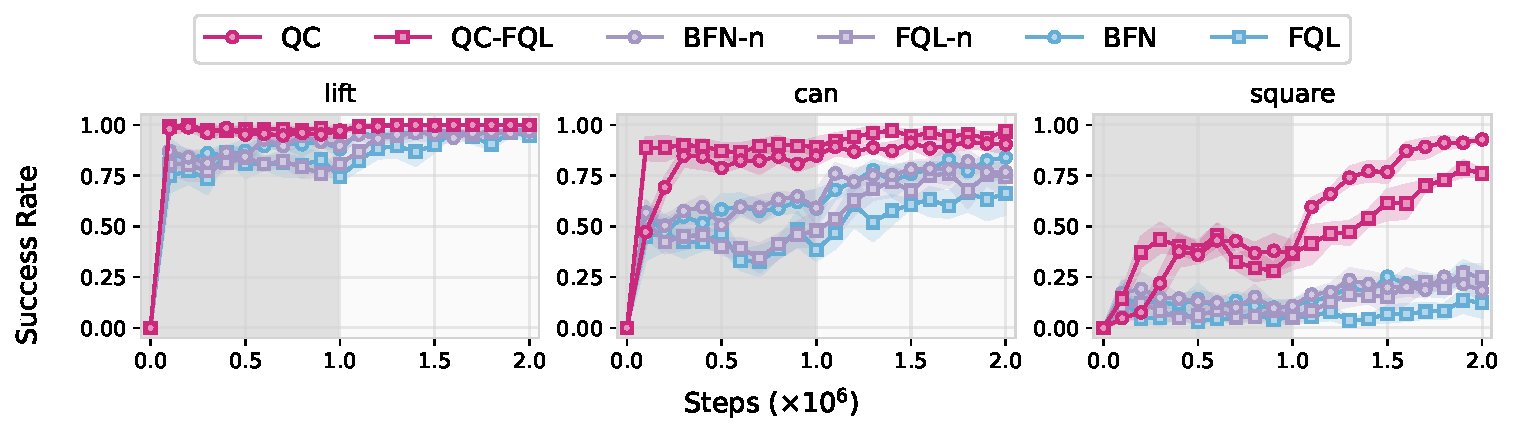
\includegraphics[width=\linewidth]{figures/robomimic-all.pdf}
    \caption{\textbf{Full robomimic ablation by task.} For each method on each task, we use 5 seeds.}
    \label{fig:full-robomimic}
\end{figure}

\subsection{How computationally efficient is Q-chunking?}
In \cref{fig:run-time}, we report the runtime for our approach and our baselines on a representative task \texttt{cube-triple-task1}. In general, \hourpurple{QC-FQL} has a comparable run-time as our baselines (e.g., \hourblue{FQL} and \hourblue{RLPD}) for both offline and online. \hourpurple{QC} is slower for offline training as it requires sampling 32 actions for each training example for the agent update (\hourblue{BFN} is faster because it only needs to sample 4 actions). For online training, we are doing one gradient update per environment step, and it makes \hourpurple{QC} only around 50\% more expensive than other methods.

\begin{figure}[H]
    \centering
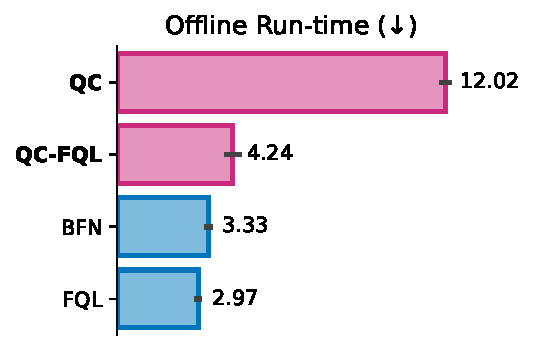
\includegraphics[width=0.48\linewidth]{figures/run-time-offline.pdf}
\label{fig:run-time-offline}
\hfill
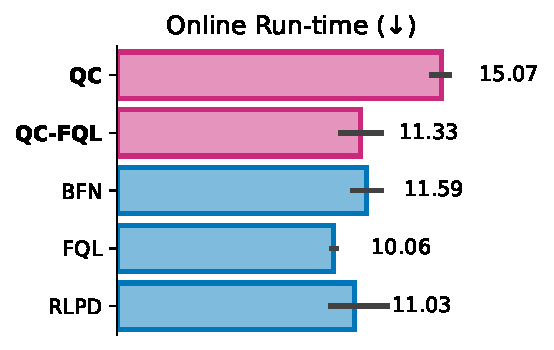
\includegraphics[width=0.48\linewidth]{figures/run-time-online.pdf}
\caption{\footnotesize \textbf{How long does each method take for one step in milliseconds.} Left: offline. Right: online (one agent training step and an environment step). The runtime is measured using the default hyperparameters in our paper on \texttt{cube-triple-task1} on a single RTX-A5000.}
\label{fig:run-time}
\end{figure}



